\chapter{Spectral Condensation}
When given a real-space representation of a flux surface, e.g., from field line tracing,
the question arises how to transform this set of points into Fourier coefficients suitable for use in VMEC.
The toroidal angle $\zeta$ is fixed by definition to be the cylindrical angle.
Tangential freedom remains in the definition of the poloidal angle,
which can be exploited to make the most economic use of the available, finite, Fourier coefficients used in the computation.
This process is called spectral condensation~\cite{hirshman_meier_1985}.

For the moment, the focus is on one-dimensional Fourier series
that describe the shape $(x,y)$ of a single flux surface in one poloidal cut
parameterized by the poloidal coordinate $\theta$:
\begin{align}
  x(\theta) =&\, \sum\limits_{m=0}^{m_\textrm{max}} x_m \cos(m \theta) \label{eqn:x_of_theta} \\
  y(\theta) =&\, \sum\limits_{m=0}^{m_\textrm{max}} y_m \sin(m \theta) \label{eqn:y_of_theta}
\end{align}
with Fourier coefficients $x_m, y_m$ for $x, y$, respectively, up to some maximum poloidal mode number $m_\textrm{max}$.
Note that above series assume stellarator symmetry.
The extension to asymmetric boundaries can be performed by including additional coefficients and basis functions
as described in the previous chapter. This is omitted here for a clearer focus on the subject of spectral condensation.

\FloatBarrier
\section{Spectral Width}
The power spectrum $S_p(m)$ of this description of the surface is defined as:
\begin{equation}
 S_p(m) = m^p (x_m^2 + y_m^2)
\end{equation}
where $p \geq 0$.
Then, a $q$-moment of $S_p(m)$ is introduced and this leads to the spectral width $M$:
\begin{equation}
 M(p,q) = \frac{\sum\limits_{m=1}^{m_\textrm{max}} m^q S_p(m)}
               {\sum\limits_{m=1}^{m_\textrm{max}}     S_p(m)}
        = \frac{\sum\limits_{m=1}^{m_\textrm{max}} m^{p+q} (x_m^2 + y_m^2)}
               {\sum\limits_{m=1}^{m_\textrm{max}} m^p     (x_m^2 + y_m^2)} \, . \label{eqn:M}
\end{equation}
The quantity $M$ measures the spectral extent of the Fourier series that describes the flux surface shape via $x_m$ and $y_m$ for $q>0$.

A given set of real-space points $(x_i, y_i)$ for $i=1, 2, ..., n_\theta$ is to be described by a spectrally condensed Fourier series.
This implies that not only the corresponding poloidal coordinates $\theta_i$ must be inferred,
but also the Fourier coefficients $x_m, y_m$ themselves are to be varied to yield a description of the surface
that at the same time is spectrally condensed with respect to the Fourier coefficients and simultaneously fits the given real-space points well.
Changes in the definition of the poloidal angle thus not only imply a change in the Fourier coefficients
but also in the values of the $\theta_i$ that correspond to prescribed real-space locations.
However, the changes in the Fourier coefficients must comply with the requirement that only the poloidal coordinate changes.
This implies that variations $\delta u$ in the poloidal coordinate must translate into purely tangential variations of the coodinates:
\begin{align}
 \delta x =&\, \frac{\partial x}{\partial \theta} \delta u \label{eqn:delta_x} \\
 \delta y =&\, \frac{\partial y}{\partial \theta} \delta u \label{eqn:delta_y} \, .
\end{align}
The corresponding changes in the Fourier coefficients that describe the surface is then obtained by Fourier-transforming the variations $\delta x$ and $\delta y$:
\begin{align}
 \delta x_m =&\, \oint \cos(m \theta) \underbrace{\frac{\partial x}{\partial \theta} \delta u}_{= \delta x} \,\mathrm{d}\theta \label{eqn:delta_x_m} \\
 \delta y_m =&\, \oint \sin(m \theta) \underbrace{\frac{\partial y}{\partial \theta} \delta u}_{= \delta y} \,\mathrm{d}\theta \label{eqn:delta_y_m} \, .
\end{align}
The changes in each of the Fourier coefficients $\delta x_m$ and $\delta y_m$ lead to a corresponding change $\delta M$ in the spectral width $M$:
\begin{equation}
 \delta M = \sum\limits_{m=1}^{m_\textrm{max}} \left[
    \frac{\partial M}{\partial x_m} \delta x_m
  + \frac{\partial M}{\partial y_m} \delta y_m \right] \, . \label{eqn:delta_M}
\end{equation}
For a fixed $m$, the partial derivatives of $M$ are obtained via the quotient rule, slightly re-arranged from the usual form:
\begin{equation}
 \left(\frac{u}{v}\right)' = \frac{u'v - u v'}{v^2} = \frac{1}{v}\left(u' - \frac{u}{v} \, v'\right)
\end{equation}
for a ratio of two functions $u$ and $v$ corresponding to the numerator and the denominator in $M$ here.
Application of this to the partial derivatives of $M$ leads to:
\begin{align}
 \frac{\partial M}{\partial x_m} =&\, \frac{1}{\sum\limits_{\tilde{m}=1}^{m_\textrm{max}} S_p(\tilde{m})}
     \Biggl( 2 m^{p+q} x_m - \underbrace{\frac{\sum\limits_{\tilde{m}=1}^{m_\textrm{max}} \tilde{m}^q S_p(\tilde{m})}
                                              {\sum\limits_{\tilde{m}=1}^{m_\textrm{max}}             S_p(\tilde{m})}}_{= M} 2 m^p x_m \Biggr)
                                 = \frac{2 m^p (m^q - M) x_m}{\sum\limits_{\tilde{m}=1}^{m_\textrm{max}} S_p(\tilde{m})} \label{eqn:dMdxm} \\
 \frac{\partial M}{\partial y_m} =&\, \frac{1}{\sum\limits_{\tilde{m}=1}^{m_\textrm{max}} S_p(\tilde{m})}
     \Biggl( 2 m^{p+q} y_m - \underbrace{\frac{\sum\limits_{\tilde{m}=1}^{m_\textrm{max}} \tilde{m}^q S_p(\tilde{m})}
                                              {\sum\limits_{\tilde{m}=1}^{m_\textrm{max}}             S_p(\tilde{m})}}_{= M} 2 m^p y_m \Biggr)
                                 = \frac{2 m^p (m^q - M) y_m}{\sum\limits_{\tilde{m}=1}^{m_\textrm{max}} S_p(\tilde{m})} \label{eqn:dMdym} \, .
\end{align}
These expressions can be inserted into the variation of $M$ in \eqn{delta_M}.
For convenience, the common denominator in \eqn{dMdxm} and \eqn{dMdym} is pulled to the front:
\begin{align}
 \delta M \sum\limits_{m=1}^{m_\textrm{max}} S_p(m)
 =&\, 2 \sum\limits_{m=1}^{m_\textrm{max}} \left[
      \left( m^p(m^q - M) x_m \delta x_m \right)
    + \left( m^p(m^q - M) y_m \delta y_m \right)
 \right] \, .
\end{align}
A common factor $f(m)$ is identified:
\begin{equation}
 f(m) = m^p (m^q - M) \, .
\end{equation}
Now the variations in the Fourier coefficients from \eqn{delta_x_m} and \eqn{delta_y_m} can be inserted:
\begin{equation}
 \delta M \sum\limits_{m=1}^{m_\textrm{max}} S_p(m)
 = 2 \sum\limits_{m=1}^{m_\textrm{max}} \left[
     f(m) x_m \oint \cos(m \theta) \frac{\partial x}{\partial \theta} \delta u \,\mathrm{d}\theta \\
   + f(m) y_m \oint \sin(m \theta) \frac{\partial y}{\partial \theta} \delta u \,\mathrm{d}\theta
 \right] \, .
\end{equation}
The integrals and the sums can be swapped:
\begin{equation}
 \delta M \sum\limits_{m=1}^{m_\textrm{max}} S_p(m)
 = 2 \oint \left[
      \sum\limits_{m=1}^{m_\textrm{max}} f(m) x_m \cos(m \theta) \frac{\partial x}{\partial \theta}
    + \sum\limits_{m=1}^{m_\textrm{max}} f(m) y_m \sin(m \theta) \frac{\partial y}{\partial \theta}
 \right] \delta u \,\mathrm{d}\theta \, .
\end{equation}
A few short-hand notations are introduced:
\begin{align}
 X(\theta) =&\, \sum\limits_{m=1}^{m_\textrm{max}} f(m) x_m \cos(m \theta) \\
 Y(\theta) =&\, \sum\limits_{m=1}^{m_\textrm{max}} f(m) y_m \sin(m \theta) \\
 I(\theta) =&\, X(\theta) \frac{\partial x}{\partial \theta} + Y(\theta) \frac{\partial y}{\partial \theta}
\end{align}
to finally arrive at:
\begin{equation}
 \delta M \sum\limits_{m=1}^{m_\textrm{max}} S_p(m)
 = 2 \oint I(\theta) \delta u \,\mathrm{d}\theta \, . \label{eqn:var_M}
\end{equation}

\FloatBarrier
\section{Curve Fitting}
Recall that the aim of this is to obtain a spectrally condensed Fourier representation
of a set of points $(x_i, y_i)$ using Fourier series for $x(\theta)$ and $y(\theta)$ as given in \eqn{x_of_theta} and \eqn{y_of_theta}
and a set of poloidal coordinates $\theta_i$ for each of the $i$ points to be represented.
For any trial set of parameters $\boldsymbol{\xi} = \{x_m, y_m, \theta_i | m=0,1,...,m_\textrm{max}, i=1, 2, ..., n_\theta \}$,
the fit to the given points can be quantified by the sum of squared deviations, also called the \textit{curve energy}:
\begin{align}
 W_c =&\, \frac{1}{2} \sum\limits_{i=1}^{n_\theta}
          \left\{ \left[ x(\theta_i) - x_i \right]^2 + \left[ y(\theta_i) - y_i \right]^2 \right\} \nonumber \\
     =&\, \frac{1}{2} \sum\limits_{i=1}^{n_\theta} \left\{
          \left[ \left(\sum\limits_{m=0}^{m_\textrm{max}} x_m \cos(m \theta_i) \right) - x_i \right]^2
        + \left[ \left(\sum\limits_{m=0}^{m_\textrm{max}} y_m \sin(m \theta_i) \right) - y_i \right]^2 \right\} \, . \label{eqn:Wc}
\end{align}
Corresponding forces on the parameters can be derived when $W_c$ is thought of as an energy:
\begin{equation}
 \mathbf{F} = - \nabla W_c = - \left\{
   \frac{\partial W_c}{\partial x_m},
   \frac{\partial W_c}{\partial y_m},
   \frac{\partial W_c}{\partial \theta_i} \right\} \, .
\end{equation}
The force components on the Fourier coefficients are:
\begin{align}
 F^x_m =&\, - \frac{\partial W_c}{\partial x_m} = - \sum\limits_{i=1}^{n_\theta} \left( x(\theta_i) - x_i \right)
   \underbrace{\cos(m \theta_i)}_{=\partial x(\theta_i) / \partial x_m} \\
 F^y_m =&\, - \frac{\partial W_c}{\partial y_m} = - \sum\limits_{i=1}^{n_\theta} \left( y(\theta_i) - y_i \right)
   \underbrace{\sin(m \theta_i)}_{=\partial y(\theta_i) / \partial y_m}
\end{align}
and the force components on the $\theta_i$ are:
\begin{equation}
   F^\theta_i
 = - \frac{\partial W_c}{\partial \theta_i}
 = - \left[  \left( x(\theta_i) - x_i \right) \frac{\partial x}{\partial \theta}(\theta_i)
           + \left( y(\theta_i) - y_i \right) \frac{\partial y}{\partial \theta}(\theta_i) \right] \, .
\end{equation}
The Jacobian matrix of this system is a $(3 \times 3)$-block matrix $\partial \mathbf{F} / \partial \boldsymbol{\xi}$ with the following layout:
\begin{align}
  \frac{\partial \mathbf{F}}{\partial \boldsymbol{\xi}}
  = \begin{pmatrix}
      \dfrac{\partial F^x_m     }{\partial x_{m'}} & \dfrac{\partial F^x_m     }{\partial y_{m'}} & \dfrac{\partial F^x_m     }{\partial \theta_i} \\[2ex]
      \dfrac{\partial F^y_m     }{\partial x_{m'}} & \dfrac{\partial F^y_m     }{\partial y_{m'}} & \dfrac{\partial F^y_m     }{\partial \theta_i} \\[2ex]
      \dfrac{\partial F^\theta_i}{\partial x_m   } & \dfrac{\partial F^\theta_i}{\partial y_m   } & \dfrac{\partial F^\theta_i}{\partial \theta_i}
    \end{pmatrix} \, .
\end{align}
It consists of the following elements:
\begin{align}
 \frac{\partial F^x_m}{\partial x_{m'}} =&\, - \sum\limits_{i=1}^{n_\theta} \cos(m' \theta_i) \cos(m \theta_i) \label{eqn:dFxmdxm}\\
 \frac{\partial F^x_m}{\partial y_{m'}} =&\, 0 \\
 \frac{\partial F^x_m}{\partial \theta_i} =&\, - \left[
     \frac{\partial x(\theta_i)}{\partial \theta_i} \cos(m \theta_i)
   - \left( x(\theta_i) - x_i \right) m \sin(m \theta_i) \right] \\
 \frac{\partial F^y_m}{\partial x_{m'}} =&\, 0 \\
 \frac{\partial F^y_m}{\partial y_{m'}} =&\, - \sum\limits_{i=1}^{n_\theta} \sin(m' \theta_i) \sin(m \theta_i) \label{eqn:dFymdym} \\
 \frac{\partial F^y_m}{\partial \theta_i} =&\, - \left[
     \frac{\partial y(\theta_i)}{\partial \theta_i} \sin(m \theta_i)
   + \left( y(\theta_i) - y_i \right) m \cos(m \theta_i) \right] \\
 \frac{\partial F^\theta_i}{\partial x_m} =&\, \frac{\partial F^x_m}{\partial \theta_i} \\
 \frac{\partial F^\theta_i}{\partial y_m} =&\, \frac{\partial F^y_m}{\partial \theta_i} \\
 \frac{\partial F^\theta_i}{\partial \theta_i} =&\, - \left[
     \left( \frac{\partial x(\theta_i)}{\partial \theta_i} \right)^2 + \left( x(\theta_i) - x_i \right) \frac{\partial^2 x(\theta_i)}{\partial \theta_i^2}
   + \left( \frac{\partial y(\theta_i)}{\partial \theta_i} \right)^2 + \left( y(\theta_i) - y_i \right) \frac{\partial^2 y(\theta_i)}{\partial \theta_i^2}
   \right] \label{eqn:dFthetadTheta}
\end{align}
where $m, m' \in [0, m_\textrm{max}]$ and $i, i' \in [1, n_\theta]$.
A sharp look reveals that the Jacobian of the curve fit forces is symmetric and relatively sparse;
note that for $i' \neq i$, $\partial F^\theta_i/\partial \theta_{i'} = 0$.

Two exemplary cases are investigated in the following.
They are the D-shaped and the bean-shaped examples from the DESCUR article~\cite{hirshman_meier_1985}.
The Jacobian matrix for each of these cases is depicted in Fig.~\ref{fig:boundary_jacobians}.
\begin{figure}[h]
  \centering
  \begin{minipage}[b]{0.49\textwidth}
    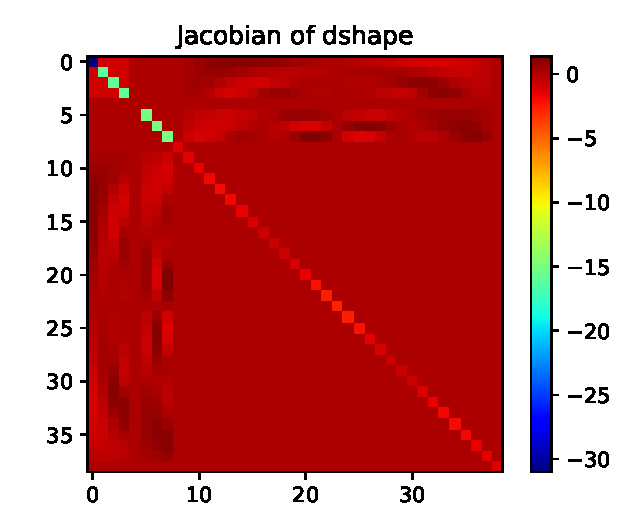
\includegraphics[width=\textwidth]{img/dshape_jac.pdf}
  \end{minipage}
  \hfill
  \begin{minipage}[b]{0.49\textwidth}
    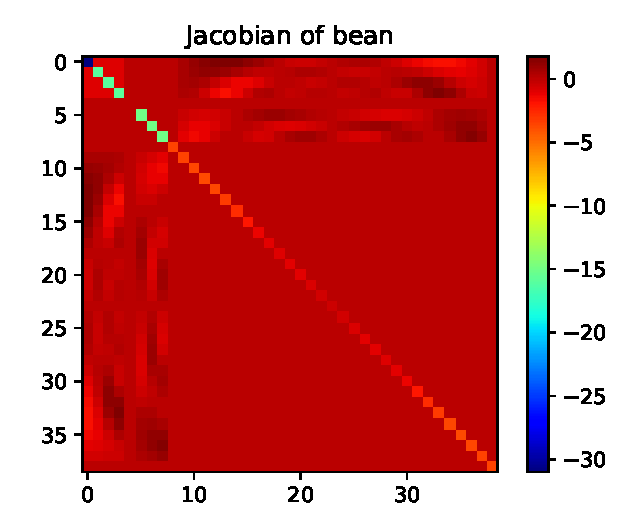
\includegraphics[width=\textwidth]{img/bean_jac.pdf}
  \end{minipage}
  \caption{Curve fit Jacobian matrix of a D-shaped and a bean-shaped boundary.}
  \label{fig:boundary_jacobians}
\end{figure}
It is evident that these matrices are approximately diagonal.
This is true for the upper left $(2 \times 2)$-block matrix (the forces on the Fourier coefficients due to changes in the Fourier coefficients)
since the orthogonality of the Fourier basis (see \eqn{ortho_fourier_basis}) ensures that all terms in \eqn{dFxmdxm} for $m \neq m'$
and all terms in \eqn{dFymdym} for $m \neq m'$ are approximately zero.
Also, as mentioned above, the lower right block is diagonal by definition, as seen in \eqn{dFthetadTheta}.

According to Ref.~\cite{gill_murray_wright}, the maximum eigenvalue of a real, symmetric matrix $\mathbf{A}$ can be computed as:
\begin{equation}
 \lambda_\textrm{max} = \max_{x \neq 0} \frac{x^T \mathbf{A} x}{x^T x} = \max_{||x|| = 1} x^T \mathbf{A} x \, .
\end{equation}
Any real symmetric $(n \times n)$ matrix $\mathbf{A}$ can be diagonalized into a form
\begin{equation}
  \mathbf{A} = \mathbf{U}^T \mathbf{\Lambda} \mathbf{U}
\end{equation}
where $\mathbf{U}$ is an orthonormal matrix and $\mathbf{\Lambda} = \mathrm{diag}\left( \lambda_1, \lambda_2, ..., \lambda_n \right)$ is the diagonal matrix
of eigenvalues $\lambda_i$ of $\mathbf{A}$.

The Jacobian matrix of the curve-fitting problem is approximately diagonal.
Therefore, the maximum eigenvalue of the Jacobian matrix approximately corresponds to the maximum diagonal element in this matrix.
The maximum element of the Jacobian matrix is located at the $(0,0)$ index and corresponds to $\partial F^x_0 / \partial x_0$, leading to:
\begin{equation}
  \lambda_\textrm{max} = \left| \frac{\partial F^x_0}{\partial x_0} \right|
  = \sum\limits_{i=1}^{n_\theta} \underbrace{\cos(0 \theta_i)}_{=1} \underbrace{\cos(0 \theta_i)}_{=1} = n_\theta \, . \label{eqn:max_eigenvalue_jac}
\end{equation}
This can be understood also intuitively.
The eigenvalues of the Jacobian matrix correspond to the changes in the ``net'' force of the curve fit problem
when any of the free parameters is changed.
Any change in $x_0$ corresponds to a radial shift of \underline{all} points simultaneously.
The curve-fit forces can be visualized by fictional rubber bands between the points to fit $(x_i, y_i)$ and the model points $(x(\theta_i), y(\theta_i))$.
For the two demo cases mentioned above, this is illustrated in Fig.~\ref{fig:rubber_bands_jac}.
\begin{figure}[h]
  \centering
  \begin{minipage}[b]{0.49\textwidth}
    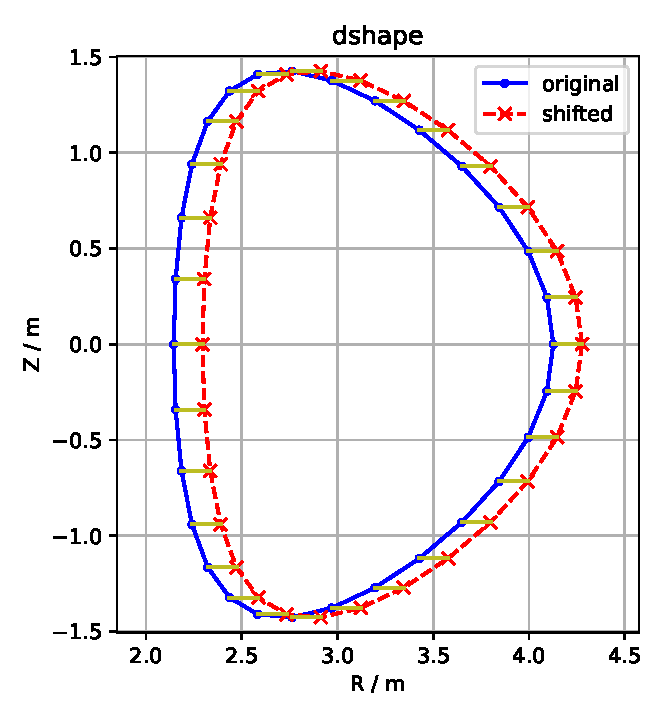
\includegraphics[width=0.74\textwidth]{img/dshape.pdf}
  \end{minipage}
  \hfill
  \begin{minipage}[b]{0.49\textwidth}
    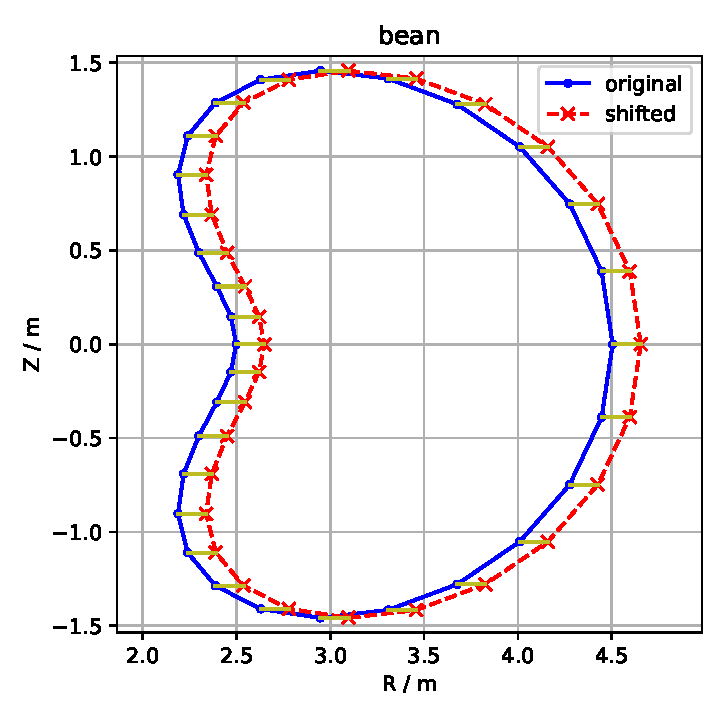
\includegraphics[width=0.8\textwidth]{img/bean.pdf}
  \end{minipage}
  \caption{A D-shaped and a bean-shaped boundary in the original shape and for a radial shift of 5~\% of their major radius.
           The yellow lines visualize fictional rubber bands between the original points and the shifted model points.}
  \label{fig:rubber_bands_jac}
\end{figure}
None of the other free parameters has such a global effect on the forces between the original points and the model points
and thus, for each rubber band (with assumed unit spring constant) a unit restoring force acts on $x_0$, for a total of $n_\theta$
unit force contributions to $F^x_0$ and (since this part of the model is linear) also to $\partial F^x_0 / \partial x_0$.
An eigendecomposition of the two Jacobian matrices was computed to verify the simplifying assumptions above.
The maximum eigenvalue of the Jacobian in the D-shaped case was $\lambda_\textrm{max, D} = 31.72$
and the maximum eigenvalue of the Jacobian in the bean-shaped case was $\lambda_\textrm{max, bean} = 32.31$.
These two numerical values have been obtained for $n_\theta = 31$ individual points around the circumference of the shapes
and are deemed sufficiently close to the approximated value in \eqn{max_eigenvalue_jac}.

\FloatBarrier
\section{Spectral Condensation Forces}
The energy functional is augmented to include an additional term related to the spectral width,
leading to the Lagrangian of the problem:
\begin{equation}
  W = W_c + \epsilon M
\end{equation}
where $\epsilon$ is a Lagrange multiplier yet to be determined.
The variation in energy due to a tangential displacement~$\delta u$ is:
\begin{equation}
  \delta W = \delta W_c + \epsilon \delta M
\end{equation}
and it follows with $\delta M$ from \eqn{var_M}:
\begin{equation}
  \delta W = \delta W_c + \frac{2 \epsilon}{\sum\limits_{m=1}^{m_\textrm{max}} S_p(m)} \oint I(\theta) \delta u \,\mathrm{d}\theta \, .
\end{equation}
The Lagrange multiplier~$\epsilon$ is rescaled according to:
\begin{equation}
  \epsilon_m = \begin{cases}
                 \epsilon / \sum\limits_{\tilde{m}=1}^{m_\textrm{max}} S_p(\tilde{m})  & m > 0 \\
                 0                                                                     & m = 0
               \end{cases}
\end{equation}
which leads to:
\begin{equation}
  \delta W = \delta W_c + 2 \epsilon_m \oint I(\theta) \delta u \,\mathrm{d}\theta \, .
\end{equation}

\FloatBarrier
\section{A Constrained Optimization Problem}
The task of finding a spectrally condensed Fourier series to describe a plane curve
represented by (randomly sampled) points along the curve can be treated as a constrained optimization problem:
\begin{align}
  \min M(\hat{x}_m, \hat{y}_m) \\
  \textrm{s.t. } W_\mathrm{c} (\hat{x}_m, \hat{y}_m, \theta_i) = 0
\end{align}
The non-linear objective function to be minimized is chosen to be the spectral width from \eqn{M}.
Note that the optimization routine is fed with the value of $M-1$, since $M$ cannot get lower than 1
and it is deemed useful to incorporate this information,
since the path taken by the optimizer in parameter space might depend on the actual value of the objective function.
The non-linear equality constraint is that the curve energy $W_\mathrm{c}$ from (\eqn{Wc}) vanishes.

The problem of finding the Fourier coefficients $\hat{x}_m$ and $\hat{y}_m$ as well as the discrete
tangential parameter values $\theta_i$ has large amounts of local minima, since for tiny changes in any of the Fourier coefficients
all $\theta_i$ would have to change in an ordered manner simultaneously.
This can (to an extent) be compensated by preconditioning, but the basic problem remains.

Here, a Fourier parameterization is chosen for the modulation $\lambda$ of the tangential parameter,
which is added to a linearly-increasing fixed background coordinate $\theta$:
\begin{align}
 \theta_i =& 2 \pi \frac{i}{N-1} \\
 \Omega_i =& \theta_i + \lambda(\theta_i)
\end{align}
for $i = 0, 1, ..., (N-1)$ with
\begin{equation}
 \lambda(\theta) = \sum_{m=1}^{m^\lambda} \hat{\lambda}_m \sin(m \theta) \, .
\end{equation}
The number of Fourier coefficients for $\lambda$, $m^\lambda$, is chosen as $m^\lambda = \lfloor \frac{N}{2} \rfloor$,
so that the full amount of information contained in the $\theta_i$ can be representated by the $\hat{\lambda}_m$.
Here, stellarator (equivalent to up-down) symmetry is assumed.

The Fourier series of $x$ and $y$ are then evaluated at the parameter $\Omega$:
\begin{align}
 x(\theta_i) =& \sum_{m=0}^{m^\mathrm{XY}} \hat{x}_m \cos(m \Omega_i) = \sum_{m=0}^{m^\mathrm{XY}} \hat{x}_m \cos(m \left[\theta_i + \lambda(\theta_i) \right]) \\
 y(\theta_i) =& \sum_{m=1}^{m^\mathrm{XY}} \hat{y}_m \sin(m \Omega_i) = \sum_{m=1}^{m^\mathrm{XY}} \hat{y}_m \sin(m \left[\theta_i + \lambda(\theta_i) \right]) \, .
\end{align}
The number of Fourier coefficients for $x$ and $y$, $m^\mathrm{XY}$, is generally chosen much smaller than $m^\lambda$.
Typical values are defined by the Fourier resolution used in a subsequently used MHD equilibrium code,
where the Fourier coefficients of the curve geometry are used to specify the shape of flux surfaces.
For VMEC, this would correspond to $m^\mathrm{XY} \lesssim 12$.

Analytical first- and second-order derivatives are now derived for both the objective function and the constraint.
They will be used by the non-linear optimization algorithm later on.

It turns out nicely that the Hessian matrices are symmetric.
This is due to the symmetry of both the constraint and the objective wrt. swapping $x$ and $y$.

The free parameters in this model are then $\hat{x}_m$, $\hat{y}_m$ and $\hat{\lambda}_m$.
The objective function $M$ only depends on $\hat{x}_m$ and $\hat{y}_m$ and its gradient is thus given fully by \eqn{dMdxm} and \eqn{dMdym}.
Here and below, $m>0$ and $m'>0$ are assumed.
The constraint function $W_\mathrm{c}$ depends on all free parameters and its gradient is given below:
\begin{align}
  \frac{\partial W_c}{\partial x(\Omega_i)}          =&\, x(\Omega_i) - x_i \\
  \frac{\partial W_c}{\partial y(\Omega_i)}          =&\, y(\Omega_i) - y_i \, ,
\end{align}
going on:
\begin{align}
  \frac{\partial x(\Omega_i)}{\partial \hat{x}_m}    =&\, \cos( m \Omega_i ) \\
  \frac{\partial x(\Omega_i)}{\partial \hat{y}_m}    =&\, 0                  \\
  \frac{\partial y(\Omega_i)}{\partial \hat{x}_m}    =&\, 0                  \\
  \frac{\partial y(\Omega_i)}{\partial \hat{y}_m}    =&\, \sin( m \Omega_i )
\end{align}
and furthermore:
\begin{align}
  \frac{\partial x(\Omega_i)}{\partial \Omega_i}     =&\,          -    \sum_{m=1}^{m^\mathrm{XY}} \hat{x}_m m \sin(m \Omega_i) \\
  \frac{\partial y(\Omega_i)}{\partial \Omega_i}     =&\, \phantom{-}\, \sum_{m=1}^{m^\mathrm{XY}} \hat{y}_m m \cos(m \Omega_i) \\
  \frac{\partial^2 x(\Omega_i)}{\partial \Omega_i^2} =&\, - \sum_{m=1}^{m^\mathrm{XY}} \hat{x}_m m^2 \cos(m \Omega_i) \\
  \frac{\partial^2 y(\Omega_i)}{\partial \Omega_i^2} =&\, - \sum_{m=1}^{m^\mathrm{XY}} \hat{y}_m m^2 \sin(m \Omega_i) \\
  \frac{\partial \Omega_i}{\partial \hat{\lambda}_m} =&\, \sin( m \theta_i ) \, .
\end{align}
Some second-order derivatives are useful later on:
\begin{align}
  \frac{\partial^2 W_c}{\partial \hat{x}_m \partial x(\Omega_i)}
  =&\, \frac{\partial x(\Omega_i)}{\partial \hat{x}_m}
  =    \cos( m \Omega_i ) \\
  \frac{\partial^2 W_c}{\partial \hat{y}_m \partial y(\Omega_i)}
  =&\, \frac{\partial y(\Omega_i)}{\partial \hat{y}_m}
  =    \sin( m \Omega_i )
\end{align}
It follows:
\begin{align}
  \frac{\partial x(\Omega_i)}{\partial \hat{\lambda}_m} =&\,          -    \left( \sum_{\tilde{m}=1}^{m^\mathrm{XY}} \hat{x}_{\tilde{m}} \tilde{m} \sin(\tilde{m} \Omega_i) \right) \sin( m \theta_i ) \\
  \frac{\partial y(\Omega_i)}{\partial \hat{\lambda}_m} =&\, \phantom{-}\, \left( \sum_{\tilde{m}=1}^{m^\mathrm{XY}} \hat{y}_{\tilde{m}} \tilde{m} \cos(\tilde{m} \Omega_i) \right) \sin( m \theta_i )
\end{align}
as well as:
\begin{align}
  \frac{\partial^2 x(\Omega_i)}{\partial \hat{x}_{m'} \partial \hat{\lambda}_m}
  =&\, \frac{\partial}{\partial \hat{x}_{m'}} \left[ - \left( \sum_{\tilde{m}=1}^{m^\mathrm{XY}} \hat{x}_{\tilde{m}} \tilde{m} \sin(\tilde{m} \Omega_i) \right) \sin( m \theta_i )  \right]
  = - m' \sin(m' \Omega_i) \sin( m \theta_i ) \\
  \frac{\partial^2 x(\Omega_i)}{\partial \hat{y}_{m'} \partial \hat{\lambda}_m}
  =&\, \frac{\partial}{\partial \hat{y}_{m'}} \left[ - \left( \sum_{\tilde{m}=1}^{m^\mathrm{XY}} \hat{x}_{\tilde{m}} \tilde{m} \sin(\tilde{m} \Omega_i) \right) \sin( m \theta_i )  \right]
  = 0 \\
  \frac{\partial^2 y(\Omega_i)}{\partial \hat{x}_{m'} \partial \hat{\lambda}_m}
  =&\, \frac{\partial}{\partial \hat{x}_{m'}} \left[\phantom{-}\, \left( \sum_{\tilde{m}=1}^{m^\mathrm{XY}} \hat{y}_{\tilde{m}} \tilde{m} \cos(\tilde{m} \Omega_i) \right) \sin( m \theta_i )  \right]
  = 0 \\
  \frac{\partial^2 y(\Omega_i)}{\partial \hat{y}_{m'} \partial \hat{\lambda}_m}
  =&\, \frac{\partial}{\partial \hat{y}_{m'}} \left[\phantom{-}\, \left( \sum_{\tilde{m}=1}^{m^\mathrm{XY}} \hat{y}_{\tilde{m}} \tilde{m} \cos(\tilde{m} \Omega_i) \right) \sin( m \theta_i )  \right]
  = \phantom{-}  m' \cos(m' \Omega_i) \sin( m \theta_i ) \\
  \frac{\partial^2 x(\Omega_i)}{\partial \hat{\lambda}_{m'} \partial \hat{\lambda}_m}
  =&\, \frac{\partial^2 x(\Omega_i)}{\partial \Omega_i^2} \frac{\partial \Omega_i}{\partial \hat{\lambda}_{m'}} \frac{\partial \Omega_i}{\partial \hat{\lambda}_m}
  = - \left( \sum_{\tilde{m}=1}^{m^\mathrm{XY}} \hat{x}_{\tilde{m}} {\tilde{m}}^2 \cos(\tilde{m} \Omega_i) \right) \sin( m' \theta_i ) \sin( m \theta_i ) \\
  \frac{\partial^2 y(\Omega_i)}{\partial \hat{\lambda}_{m'} \partial \hat{\lambda}_m}
  =&\, \frac{\partial^2 y(\Omega_i)}{\partial \Omega_i^2} \frac{\partial \Omega_i}{\partial \hat{\lambda}_{m'}} \frac{\partial \Omega_i}{\partial \hat{\lambda}_m}
  = - \left( \sum_{\tilde{m}=1}^{m^\mathrm{XY}} \hat{y}_{\tilde{m}} {\tilde{m}}^2 \sin(\tilde{m} \Omega_i) \right) \sin( m' \theta_i ) \sin( m \theta_i )
\end{align}
From above parts, the full gradient vector of the constraint can be assembled:
\begin{align}
 \frac{\partial W_c}{\partial \hat{x}_m}
  =&\, \sum_{i=0}^{N-1} \frac{\partial W_c}{\partial x(\Omega_i)} \frac{\partial x(\Omega_i)}{\partial \hat{x}_m}
  =    \sum_{i=0}^{N-1} \left( x(\Omega_i) - x_i \right) \cos( m \Omega_i ) \\
 \frac{\partial W_c}{\partial \hat{y}_m}
  =&\, \sum_{i=0}^{N-1} \frac{\partial W_c}{\partial y(\Omega_i)} \frac{\partial y(\Omega_i)}{\partial \hat{y}_m}
  =    \sum_{i=0}^{N-1} \left( y(\Omega_i) - y_i \right) \sin( m \Omega_i ) \\
\frac{\partial W_c}{\partial \hat{\lambda}_m}
 =&\, \sum_{i=0}^{N-1} \left(  \frac{\partial W_c}{\partial x(\Omega_i)} \frac{\partial x(\Omega_i)}{\partial \Omega_i}
                             + \frac{\partial W_c}{\partial y(\Omega_i)} \frac{\partial y(\Omega_i)}{\partial \Omega_i}
                       \right) \frac{\partial \Omega_i}{\partial \hat{\lambda}_m} \nonumber \\
~=&\,         \sum_{i=0}^{N-1} \Biggl[  - \left( x(\Omega_i) - x_i \right) \left( \sum_{\tilde m =1}^{m^\mathrm{XY}} \hat{x}_{\tilde{m}} \tilde{m} \sin(\tilde{m} \Omega_i) \right) \nonumber \\
~&\, \phantom{\sum_{i=0}^{N-1} \Biggl[} + \left( y(\Omega_i) - y_i \right) \left( \sum_{\tilde m =1}^{m^\mathrm{XY}} \hat{y}_{\tilde{m}} \tilde{m} \cos(\tilde{m} \Omega_i) \right) \Biggr] \sin( m \theta_i )
\end{align}
The problem at hand is fully analytic and therefore, analytical second-order derivatives of the objective as well as the constraint are derived next.
First the second-order derivatives of the objective function $M$ are considered:
\begin{align}
  \frac{\partial^2 M}{\partial \hat{x}_{m'} \partial \hat{x}_m}
  =&\, \frac{\partial}{\partial \hat{x}_{m'}} \left( \frac{\partial M}{\partial \hat{x}_m} \right)
  =    \frac{\partial}{\partial \hat{x}_{m'}} \left( \frac{2 m^p (m^q - M) \hat{x}_m}{\sum\limits_{\tilde{m}=1}^{m^\textrm{XY}} \tilde{m}^p (\hat{x}_{\tilde{m}}^2 + \hat{y}_{\tilde{m}}^2)} \right) \nonumber \\
  =&\, \frac{1}{\sum\limits_{\tilde{m}=1}^{m^\textrm{XY}} \tilde{m}^p (\hat{x}_{\tilde{m}}^2 + \hat{y}_{\tilde{m}}^2)}
       \left[                                        \frac{\partial}{\partial \hat{x}_{m'}} \Bigl( 2 m^p (m^q - M) \hat{x}_m                                                                             \Bigr)
             - \frac{\partial M}{\partial \hat{x}_m} \frac{\partial}{\partial \hat{x}_{m'}} \left( \sum\limits_{\tilde{m}=1}^{m^\textrm{XY}} \tilde{m}^p (\hat{x}_{\tilde{m}}^2 + \hat{y}_{\tilde{m}}^2) \right)
       \right] \nonumber \\
  =&\, - \frac{2}{\sum\limits_{\tilde{m}=1}^{m^\textrm{XY}} \tilde{m}^p (\hat{x}_{\tilde{m}}^2 + \hat{y}_{\tilde{m}}^2)}
         \left[ m^p \hat{x}_{m} \frac{\partial M}{\partial \hat{x}_{m'}} + {m'}^p \hat{x}_{m'} \frac{\partial M}{\partial \hat{x}_m} - m^p (m^q - M) \delta_{m m'} \right]
\end{align}
Furthermore:
\begin{align}
  \frac{\partial^2 M}{\partial \hat{y}_{m'} \partial \hat{x}_m}
  =&\, \frac{\partial}{\partial \hat{y}_{m'}} \left( \frac{\partial M}{\partial \hat{x}_m} \right)
  =    \frac{\partial}{\partial \hat{y}_{m'}} \left( \frac{2 m^p (m^q - M) \hat{x}_m}{\sum\limits_{\tilde{m}=1}^{m^\textrm{XY}} \tilde{m}^p (\hat{x}_{\tilde{m}}^2 + \hat{y}_{\tilde{m}}^2)} \right) \nonumber \\
  =&\, \frac{1}{\sum\limits_{\tilde{m}=1}^{m^\textrm{XY}} \tilde{m}^p (\hat{x}_{\tilde{m}}^2 + \hat{y}_{\tilde{m}}^2)}
       \left[- 2 m^p \hat{x}_m \frac{\partial M}{\partial \hat{y}_{m'}}
             - \frac{\partial M}{\partial \hat{x}_m} \frac{\partial}{\partial \hat{y}_{m'}} \left( \sum\limits_{\tilde{m}=1}^{m^\textrm{XY}} \tilde{m}^p (\hat{x}_{\tilde{m}}^2 + \hat{y}_{\tilde{m}}^2) \right)
       \right] \nonumber \\
  =&\, - \frac{2}{\sum\limits_{\tilde{m}=1}^{m^\textrm{XY}} \tilde{m}^p (\hat{x}_{\tilde{m}}^2 + \hat{y}_{\tilde{m}}^2)}
         \left[ m^p \hat{x}_{m} \frac{\partial M}{\partial \hat{y}_{m'}} + {m'}^p \hat{y}_{m'} \frac{\partial M}{\partial \hat{x}_m} \right]
\end{align}
Finally:
\begin{align}
  \frac{\partial^2 M}{\partial \hat{y}_{m'} \partial \hat{y}_m}
  =&\, \frac{\partial}{\partial \hat{y}_{m'}} \left( \frac{\partial M}{\partial \hat{y}_m} \right)
  =    \frac{\partial}{\partial \hat{y}_{m'}} \left( \frac{2 m^p (m^q - M) \hat{y}_m}{\sum\limits_{\tilde{m}=1}^{m^\textrm{XY}} \tilde{m}^p (\hat{x}_{\tilde{m}}^2 + \hat{y}_{\tilde{m}}^2)} \right) \nonumber \\
  =&\, \frac{1}{\sum\limits_{\tilde{m}=1}^{m^\textrm{XY}} \tilde{m}^p (\hat{x}_{\tilde{m}}^2 + \hat{y}_{\tilde{m}}^2)}
       \left[                                        \frac{\partial}{\partial \hat{y}_{m'}} \Bigl( 2 m^p (m^q - M) \hat{y}_m                                                                             \Bigr)
             - \frac{\partial M}{\partial \hat{y}_m} \frac{\partial}{\partial \hat{y}_{m'}} \left( \sum\limits_{\tilde{m}=1}^{m^\textrm{XY}} \tilde{m}^p (\hat{x}_{\tilde{m}}^2 + \hat{y}_{\tilde{m}}^2) \right)
       \right] \nonumber \\
  =&\, - \frac{2}{\sum\limits_{\tilde{m}=1}^{m^\textrm{XY}} \tilde{m}^p (\hat{x}_{\tilde{m}}^2 + \hat{y}_{\tilde{m}}^2)}
         \left[ m^p \hat{y}_{m} \frac{\partial M}{\partial \hat{y}_{m'}} + {m'}^p \hat{y}_{m'} \frac{\partial M}{\partial \hat{y}_m} - m^p (m^q - M) \delta_{m m'} \right]
\end{align}
The second-order derivatives of the constraint are considered next.
The second-order derivatives with respect to $\hat{x}_m$ and $\hat{y}_m$ are similar to the corresponding components of the curve-fit Jacobian:
\begin{align}
  \frac{\partial^2 W_\mathrm{c}}{\partial \hat{x}_{m'} \partial \hat{x}_m}
  =&\, \frac{\partial}{\partial \hat{x}_{m'}} \left( \frac{\partial W_\mathrm{c}}{\partial \hat{x}_m} \right)
  = \sum_{i=0}^{N-1} \cos( m' \Omega_i ) \cos( m \Omega_i ) \\
  \frac{\partial^2 W_\mathrm{c}}{\partial \hat{y}_{m'} \partial \hat{x}_m}
  =&\, 0 \\
  \frac{\partial^2 W_\mathrm{c}}{\partial \hat{x}_{m'} \partial \hat{y}_m}
  =&\, 0 \\
  \frac{\partial^2 W_\mathrm{c}}{\partial \hat{y}_{m'} \partial \hat{y}_m}
  =&\, \frac{\partial}{\partial \hat{y}_{m'}} \left( \frac{\partial W_\mathrm{c}}{\partial \hat{y}_m} \right)
  = \sum_{i=0}^{N-1} \sin( m' \Omega_i ) \sin( m \Omega_i )
\end{align}
Furthermore:
\begin{align}
  \frac{\partial^2 W_\mathrm{c}}{\partial \hat{x}_{m'} \partial \hat{\lambda}_m}
  =&\, \sum_{i=0}^{N-1} \frac{\partial}{\partial \hat{x}_{m'}}
                        \left(  \frac{\partial W_c}{\partial x(\Omega_i)} \frac{\partial x(\Omega_i)}{\partial \hat{\lambda}_m}
                              + \frac{\partial W_c}{\partial y(\Omega_i)} \frac{\partial y(\Omega_i)}{\partial \hat{\lambda}_m}
                       \right) \nonumber \\
  =&\, \sum_{i=0}^{N-1} \Biggl(\phantom{+}\,  \frac{\partial^2 W_c}{\partial \hat{x}_{m'} \partial x(\Omega_i)} \frac{\partial   x(\Omega_i)}{                      \partial \hat{\lambda}_m}
                               + \frac{\partial   W_c}{                      \partial x(\Omega_i)} \frac{\partial^2 x(\Omega_i)}{\partial \hat{x}_{m'} \partial \hat{\lambda}_m} \nonumber \\
~ &\, \phantom{\sum_{i=0}^{N-1} \Biggl(}\,  + \underbrace{\frac{\partial^2 W_c}{\partial \hat{x}_{m'} \partial y(\Omega_i)}}_{=0} \frac{\partial   y(\Omega_i)}{                      \partial \hat{\lambda}_m}
                               + \frac{\partial   W_c}{                      \partial y(\Omega_i)} \underbrace{\frac{\partial^2 y(\Omega_i)}{\partial \hat{x}_{m'} \partial \hat{\lambda}_m}}_{=0}
                        \Biggr) \nonumber \\
  =&\, \sum_{i=0}^{N-1} \left(  \cos(m' \Omega_i) \frac{\partial x(\Omega_i)}{\partial \Omega_i}
                              - (x(\Omega_i) - x_i) m' \sin(m' \Omega_i) \right) \sin( m \theta_i ) \label{eqn:d2WcdXmdLm}
\end{align}
as well as:
\begin{align}
  \frac{\partial^2 W_\mathrm{c}}{\partial \hat{y}_{m'} \partial \hat{\lambda}_m}
  =&\, \sum_{i=0}^{N-1} \frac{\partial}{\partial \hat{y}_{m'}}
                        \left(  \frac{\partial W_c}{\partial x(\Omega_i)} \frac{\partial x(\Omega_i)}{\partial \hat{\lambda}_m}
                              + \frac{\partial W_c}{\partial y(\Omega_i)} \frac{\partial y(\Omega_i)}{\partial \hat{\lambda}_m}
                       \right) \nonumber \\
  =&\, \sum_{i=0}^{N-1} \Biggl(\phantom{+}\,  \underbrace{\frac{\partial^2 W_c}{\partial \hat{y}_{m'} \partial x(\Omega_i)}}_{=0} \frac{\partial   x(\Omega_i)}{                      \partial \hat{\lambda}_m}
                               + \frac{\partial   W_c}{                      \partial x(\Omega_i)} \underbrace{\frac{\partial^2 x(\Omega_i)}{\partial \hat{y}_{m'} \partial \hat{\lambda}_m}}_{=0} \nonumber \\
~ &\, \phantom{\sum_{i=0}^{N-1} \Biggl(}\,  + \frac{\partial^2 W_c}{\partial \hat{y}_{m'} \partial y(\Omega_i)} \frac{\partial   y(\Omega_i)}{                      \partial \hat{\lambda}_m}
                               + \frac{\partial   W_c}{                      \partial y(\Omega_i)} \frac{\partial^2 y(\Omega_i)}{\partial \hat{y}_{m'} \partial \hat{\lambda}_m}
                        \Biggr) \nonumber \\
  =&\, \sum_{i=0}^{N-1} \left(  \sin(m' \Omega_i) \frac{\partial y(\Omega_i)}{\partial \Omega_i}
                                 + (y(\Omega_i) - y_i) m' \cos(m' \Omega_i) \right) \sin( m \theta_i ) \label{eqn:d2WcdYmdLm}
\end{align}
The second-order derivatives with respect to $\hat{\lambda}_m$ follow:
\begin{align}
  \frac{\partial^2 W_\mathrm{c}}{\partial \hat{\lambda}_{m'} \partial \hat{x}_m}
  =&\, \sum_{i=0}^{N-1} \frac{\partial}{\partial \hat{\lambda}_{m'}} \Bigl[ \left( x(\Omega_i) -  x_i \right) \cos( m \Omega_i ) \Bigr] \nonumber \\
  =&\, \sum_{i=0}^{N-1} \left[  \frac{\partial x(\Omega_i)}{\partial \hat{\lambda}_{m'}} \cos( m \Omega_i )
                               - \left( x(\Omega_i) - x_i \right) m \sin(m \Omega_i) \sin(m' \theta_i) \right] \nonumber \\
  =&\, \sum_{i=0}^{N-1} \left[   \cos( m \Omega_i ) \frac{\partial x(\Omega_i)}{\partial \Omega_i}
                               - \left( x(\Omega_i) - x_i \right) m \sin(m \Omega_i) \right] \sin(m' \theta_i) \label{eqn:d2WcdLmdXm} \\
  \frac{\partial^2 W_\mathrm{c}}{\partial \hat{\lambda}_{m'} \partial \hat{y}_m}
  =&\, \sum_{i=0}^{N-1} \frac{\partial}{\partial \hat{\lambda}_{m'}} \Bigl[ \left( y(\Omega_i) - y_i \right) \sin( m \Omega_i ) \Bigr] \nonumber \\
  =&\, \sum_{i=0}^{N-1} \left[  \frac{\partial y(\Omega_i)}{\partial \hat{\lambda}_{m'}} \sin( m \Omega_i )
                               + \left( y(\Omega_i) - y_i \right) m \cos(m \Omega_i) \sin(m' \theta_i) \right] \nonumber \\
  =&\, \sum_{i=0}^{N-1} \left[   \sin( m \Omega_i ) \frac{\partial y(\Omega_i)}{\partial \Omega_i}
                               + \left( y(\Omega_i) - y_i \right) m \cos(m \Omega_i) \right] \sin(m' \theta_i) \label{eqn:d2WcdLmdYm}
\end{align}
It is (expectedly) observed that \eqn{d2WcdXmdLm} equals \eqn{d2WcdLmdXm} and \eqn{d2WcdYmdLm} equals \eqn{d2WcdLmdYm} under exchange of $m$ and $m'$.
Finally:
\begin{align}
  \frac{\partial^2 W_\mathrm{c}}{\partial \hat{\lambda}_{m'} \partial \hat{\lambda}_m}
  =&\, \sum_{i=0}^{N-1} \frac{\partial}{\partial \hat{\lambda}_{m'}}
                        \left(  \frac{\partial W_c}{\partial x(\Omega_i)} \frac{\partial x(\Omega_i)}{\partial \hat{\lambda}_m}
                              + \frac{\partial W_c}{\partial y(\Omega_i)} \frac{\partial y(\Omega_i)}{\partial \hat{\lambda}_m}
                        \right) \nonumber \\
  =&\,          \sum_{i=0}^{N-1} \Biggl(   \phantom{+}\, \frac{\partial^2 W_c}{\partial \hat{\lambda}_{m'} \partial x(\Omega_i)} \frac{\partial   x(\Omega_i)}{                            \partial \hat{\lambda}_m}
                                                    +    \frac{\partial   W_c}{                            \partial x(\Omega_i)} \frac{\partial^2 x(\Omega_i)}{\partial \hat{\lambda}_{m'} \partial \hat{\lambda}_m} \nonumber \\
 ~ &\, \phantom{\sum_{i=0}^{N-1} \Biggl(}\,         +    \frac{\partial^2 W_c}{\partial \hat{\lambda}_{m'} \partial y(\Omega_i)} \frac{\partial   y(\Omega_i)}{                            \partial \hat{\lambda}_m}
                                                    +    \frac{\partial   W_c}{                            \partial y(\Omega_i)} \frac{\partial^2 y(\Omega_i)}{\partial \hat{\lambda}_{m'} \partial \hat{\lambda}_m}
                                 \Biggr) \nonumber \\
  =&\,          \sum_{i=0}^{N-1} \Biggl(   \phantom{+}\, \frac{\partial x(\Omega_i)}{\partial \hat{\lambda}_{m'}} \frac{\partial x(\Omega_i)}{\partial \hat{\lambda}_m}
                                                    +    (x(\Omega_i) - x_i) \frac{\partial^2 x(\Omega_i)}{\partial \hat{\lambda}_{m'} \partial \hat{\lambda}_m} \nonumber \\
 ~ &\, \phantom{\sum_{i=0}^{N-1} \Biggl(}\,         +    \frac{\partial y(\Omega_i)}{\partial \hat{\lambda}_{m'}} \frac{\partial y(\Omega_i)}{\partial \hat{\lambda}_m}
                                                    +    (y(\Omega_i) - y_i) \frac{\partial^2 y(\Omega_i)}{\partial \hat{\lambda}_{m'} \partial \hat{\lambda}_m}
                                 \Biggr) \nonumber \\
  =&\,          \sum_{i=0}^{N-1} \Biggl[
      \phantom{+}\, \left( \frac{\partial x(\Omega_i)}{\partial \Omega_i} \right)^2 + \left( x(\Omega_i) - x_i \right) \frac{\partial^2 x(\Omega_i)}{\partial \Omega_i^2} \nonumber \\
  ~&\, \phantom{\sum_{i=0}^{N-1} \Biggl[}
               +    \left( \frac{\partial y(\Omega_i)}{\partial \Omega_i} \right)^2 + \left( y(\Omega_i) - y_i \right) \frac{\partial^2 y(\Omega_i)}{\partial \Omega_i^2} \Biggr]
       \sin(m' \theta_i) \sin(m \theta_i)
\end{align}

\FloatBarrier
\newpage
\section{Direct Equal-Arclength Parameterization}
%
Kuhl and Giardina~\cite{kuhl_giardina_1982} present a method to directly and robustly compute equal-arclength parameterized
Fourier coefficients for a given closed curve in the plane.
A Python implementation of their method is available in Ref.~\cite{pyefd}.
This method has applications in two areas of Stellarator research.
First, it can be used to obtain a Fourier description of Poincare data from magnetic field line tracing.
Second, it can be used in  a 3D MHD equilibrium code to define a unique (although not optimal; see below)
poloidal angle-like coordinate/parameter.

The input data for this method is a set of points $\{(x_i, y_i)|i=0,1,..., (N-1)\}$ along a closed curve in the plane.
We define $x_N \equiv x_0$ and $y_N \equiv y_0$ for convenience.
If the geometry to be used as input is already a Fourier series, it needs to be evaluated at consecutive values
of the tangential parameter, e.g., by an inverse FFT. This would imply evaluations at equal increments of the tangential parameter,
which is not a strict necessity for the method under discussion here.
The tangential parameter $t$ is introduced as the arclength along the curve, which can be computed as follows
assuming piecewise-linear segments connecting the points given as input.

Define for $i = 0, 1, ..., (N-1)$:
\begin{align}
  \Delta x_i =&\, x_{i+1} - x_i \\
  \Delta y_i =&\, y_{i+1} - y_i \\
  \Delta t_i =&\, \sqrt{ \Delta x_i^2 + \Delta y_i^2 } \\
         t_i =&\, \begin{cases}
                    0                    &: i=0 \\
                    t_{i-1} + \Delta t_i &: \textrm{ else} \, .
                  \end{cases}
\end{align}
The total arclength or circumference of the curve $T$ is then given by:
\begin{equation}
  T = t_N = t_{N-1} + \Delta t_{N-1} \, .
\end{equation}
An angle-like tangential parameter $\theta$ can then be introduced by:
\begin{equation}
  \theta = \frac{2 \pi t}{T}
\end{equation}
for disrete values $\theta_i$:
\begin{equation}
  \theta_i = \frac{2 \pi}{T} t_i \, .
\end{equation}
The points along the curve can be reconstructed from the discrete differentials $\Delta x_i$, $\Delta y_i$
and the first point $(x_0, y_0)$:
\begin{align}
  x_i =& x_0 + \sum_{k=0}^{i-1} \Delta x_k \\
  y_i =& y_0 + \sum_{k=0}^{i-1} \Delta y_k \, .
\end{align}
A piecewise-linear continuous description of the curve geometry is formulated as follows:
\begin{align}
  x(t) =&\, x_i + (t - t_i) \frac{x_{i+1} - x_i}{t_{i+1} - t_i} \nonumber \\
       =&\, x_i + (t - t_i) \frac{\Delta x_i}{\Delta t_i} \label{eqn:efd_pl_x} \\
  y(t) =&\, y_i + (t - t_i) \frac{\Delta y_i}{\Delta t_i} \, .
\end{align}
for $t_i \leq t < t_{i+1}$ and $0 \leq i < N$.
The targeted truncated Fourier description of this curve geometry is formulated as follows:
\begin{align}
  x(t) =&\, A_0 + \sum_{m=1}^{m^\mathrm{XY}} \left[   a_m \cos\left( \frac{2 \pi}{T} m t \right)
                                                    + b_m \sin\left( \frac{2 \pi}{T} m t \right) \right] \label{eqn:efd_fs_x} \\
  y(t) =&\, C_0 + \sum_{m=1}^{m^\mathrm{XY}} \left[   c_m \cos\left( \frac{2 \pi}{T} m t \right)
                                                    + d_m \sin\left( \frac{2 \pi}{T} m t \right) \right]
\end{align}
where
\begin{align}
  A_0 =&\, \frac{1}{T} \int\limits_{0}^{T} x(t) \mathrm{d}t \\
  C_0 =&\, \frac{1}{T} \int\limits_{0}^{T} y(t) \mathrm{d}t \\
  a_m =&\, \frac{2}{T} \int\limits_{0}^{T} x(t) \cos\left( \frac{2 \pi}{T} m t \right) \mathrm{d}t \label{eqn:efd_a_m} \\
  b_m =&\, \frac{2}{T} \int\limits_{0}^{T} x(t) \sin\left( \frac{2 \pi}{T} m t \right) \mathrm{d}t \\
  c_m =&\, \frac{2}{T} \int\limits_{0}^{T} y(t) \cos\left( \frac{2 \pi}{T} m t \right) \mathrm{d}t \\
  d_m =&\, \frac{2}{T} \int\limits_{0}^{T} y(t) \sin\left( \frac{2 \pi}{T} m t \right) \mathrm{d}t \, .
\end{align}
Several approaches are possible for the numerical evaluation of the Fourier integrals listed above
to obtain the Fourier coefficients $A_0$, $C_0$ and $a_m$, $b_m$, $c_m$ and $d_m$
up to a maximum poloidal mode number $m^\mathrm{XY}$.

\subsection{Trapezoidal Quadrature}
Direct application of the trapezoidal rule to above Fourier integrals leads to:
\begin{align}
  A_0 =&\, \frac{1}{T} \int\limits_{0}^{T} x(t) \mathrm{d}t \nonumber \\
      \approx&\, \frac{1}{T} \sum_{i=0}^{N-1} \frac{x_i + x_{i+1}}{2} \delta t_i \nonumber \\
      =&\, \frac{1}{2 T} \sum_{i=0}^{N-1} (x_i + x_{i+1}) \delta t_i
\end{align}
and
\begin{align}
  a_m =&\, \frac{2}{T} \int\limits_{0}^{T} x(t) \cos\left( \frac{2 \pi}{T} m t \right) \mathrm{d}t \nonumber \\
      \approx&\, \frac{\bcancel{2}}{T} \sum_{i=0}^{N-1} \frac{1}{\bcancel{2}} \left[   x_i     \cos\left( \frac{2 \pi}{T} m t_i     \right)
                                                                                     + x_{i+1} \cos\left( \frac{2 \pi}{T} m t_{i+1} \right) \right] \Delta t_i \nonumber \\
      =&\, \frac{1}{T} \sum_{i=0}^{N-1} \left[   x_i     \cos\left( \frac{2 \pi}{T} m t_i     \right)
                                               + x_{i+1} \cos\left( \frac{2 \pi}{T} m t_{i+1} \right) \right] \Delta t_i
\end{align}
as well as
\begin{align}
  b_m =&\, \frac{2}{T} \int\limits_{0}^{T} x(t) \sin\left( \frac{2 \pi}{T} m t \right) \mathrm{d}t \nonumber \\
      \approx&\, \frac{\bcancel{2}}{T} \sum_{i=0}^{N-1} \frac{1}{\bcancel{2}} \left[   x_i     \sin\left( \frac{2 \pi}{T} m t_i     \right)
                                                                                     + x_{i+1} \sin\left( \frac{2 \pi}{T} m t_{i+1} \right) \right] \Delta t_i \nonumber \\
      =&\, \frac{1}{T} \sum_{i=0}^{N-1} \left[   x_i     \sin\left( \frac{2 \pi}{T} m t_i     \right)
                                               + x_{i+1} \sin\left( \frac{2 \pi}{T} m t_{i+1} \right) \right] \Delta t_i \, .
\end{align}
The remaining coefficients $C_0$, $c_m$ and $d_m$ are obtained by replacing $x$ with $y$ in above expressions, respectively.
The computational cost for this method is comparably low.
A significant factor of oversampling is required to achieve an accurate match with the original point data
from the Fourier representation obtained using trapezoidal quadrature.

\subsection{Analytical Integration over Piecewise-Linear Segments}
This approach is presented by Kuhl and Giardina in their article~\cite{kuhl_giardina_1982}.
The key idea is to evaluate the Fourier integrals for $A_0$, ..., $d_m$ analytically for assumed piecewise-linear segments connecting the given input points.
It might seem counterintuitive to explicitly put straight segments into the model when trying to fit curved geometries.
(Note that Kuhl and Giardina applied this method to chain codes, where linear segments are desired.)
When operating close to the Nyquist limit, there are not enough modes present to force the Fourier representation straight in between sample points.
When operating way below the Nyquist limit (i.e., more points than needed for a given number of Fourier coefficients according to the sampling theorem),
the implied line segments are much shorter than the wavelength of the highest mode to be reconstructed, so no artificial straightening happens.
It is only possible to obtain straight segments from the Fourier representation when reconstructing way more Fourier modes thatn the Nyquist theorem
would allow for based on the given number of input points. This is desired and intended by Kuhl and Giardina for their application
of representing chain codes, but not a useful modus operandi in the context of this work.

There are (at least) two different ways to derive the results in Ref.~\cite{kuhl_giardina_1982}.
The first one is to express both $x(t)$ and $\partial x/\partial t$ as Fourier series
and perform analytical integration in the Fourier integrals for $\partial x/\partial t$, then equate coefficients.
This is the way chosen by Kuhl and Giardina originally.
It is repeated here due to typographic errors in the original article.

A new Fourier series is introduced for $\partial x/\partial t$:
\begin{equation}
  \frac{\partial x}{\partial t}(t) = \sum_{m=1}^{m^\mathrm{XY}} \left[ \alpha_m \cos\left( \frac{2 \pi}{T} m t \right)
                                                                      + \beta_m \sin\left( \frac{2 \pi}{T} m t \right) \right]
\end{equation}
with
\begin{align}
  \alpha_m =&\, \frac{2}{T} \int\limits_0^T \frac{\partial x}{\partial t}(t) \cos\left( \frac{2 \pi}{T} m t \right) \mathrm{d}t \\
   \beta_m =&\, \frac{2}{T} \int\limits_0^T \frac{\partial x}{\partial t}(t) \sin\left( \frac{2 \pi}{T} m t \right) \mathrm{d}t \, .
\end{align}
The tangential derivative $\partial x/\partial t$ is piecewise constant for assumed straight segments between given points.
The integrals for $\alpha_m$ and $\beta_m$ can therefore be evaluated as follows:
\begin{align}
  \alpha_m =&\, \frac{2}{T} \sum_{i=0}^{N-1} \frac{\Delta x_i}{\Delta t_i} \int\limits_{t_i}^{t_{i+1}} \cos\left( \frac{2 \pi}{T} m t \right) \mathrm{d}t \nonumber \\
           =&\, \frac{\bcancel{2}}{\cancel{T}} {\color{blue} \frac{\cancel{T}}{\bcancel{2} \pi m} }
                \sum_{i=0}^{N-1} \frac{\Delta x_i}{\Delta t_i} \left[ \sin\left( \frac{2 \pi}{T} m t_{i+1} \right) - \sin\left( \frac{2 \pi}{T} m t_i \right) \right] \nonumber \\
           =&\, \frac{1}{\pi m} \sum_{i=0}^{N-1} \frac{\Delta x_i}{\Delta t_i} \left[ \sin\left( \frac{2 \pi}{T} m t_{i+1} \right) - \sin\left( \frac{2 \pi}{T} m t_i \right) \right] \\
   \beta_m =&\, \frac{2}{T} \sum_{i=0}^{N-1} \frac{\Delta x_i}{\Delta t_i} \int\limits_{t_i}^{t_{i+1}} \sin\left( \frac{2 \pi}{T} m t \right) \mathrm{d}t \nonumber \\
           =&\, - \frac{\bcancel{2}}{\cancel{T}} {\color{blue} \frac{\cancel{T}}{\bcancel{2} \pi m} }
                \sum_{i=0}^{N-1} \frac{\Delta x_i}{\Delta t_i} \left[ \cos\left( \frac{2 \pi}{T} m t_{i+1} \right) - \cos\left( \frac{2 \pi}{T} m t_i \right) \right] \nonumber \\
           =&\, \frac{-1}{\pi m} \sum_{i=0}^{N-1} \frac{\Delta x_i}{\Delta t_i} \left[ \cos\left( \frac{2 \pi}{T} m t_{i+1} \right) - \cos\left( \frac{2 \pi}{T} m t_i \right) \right] \, .
\end{align}
The terms marked blue are missing in the original article, although their final results are correct.
Note that $\partial x/\partial t$ can also be obtained by differentiation of the Fourier series for $x(t)$ from \eqn{efd_fs_x}:
\begin{align}
  \frac{\partial x}{\partial t}(t) =&\, \frac{\partial}{\partial t} \left\{
    A_0 + \sum_{m=1}^{m^\mathrm{XY}} \left[   a_m \cos\left( \frac{2 \pi}{T} m t \right)
                                            + b_m \sin\left( \frac{2 \pi}{T} m t \right) \right] \right\} \\
     =&\, \sum_{m=1}^{m^\mathrm{XY}} \left[ - a_m \frac{2 \pi m}{T} \sin\left( \frac{2 \pi}{T} m t \right)
                                            + b_m \frac{2 \pi m}{T} \cos\left( \frac{2 \pi}{T} m t \right) \right] \, .
\end{align}
Equating the two representations of $\partial x/\partial t$ we obtain:
\begin{align}
  - a_m \frac{2 \pi m}{T} =  \beta_m \Leftrightarrow&\, a_m =          -    \frac{T}{2 \pi m}  \beta_m \\
    b_m \frac{2 \pi m}{T} = \alpha_m \Leftrightarrow&\, b_m = \phantom{-}\, \frac{T}{2 \pi m} \alpha_m \, .
\end{align}
The coefficients $a_m$, $b_m$ can now be obtained by inserting the explicit forms of $\alpha_m$, $\beta_m$:
\begin{align}
  a_m =&\, \bcancel{-} \frac{T}{2 \pi m} \frac{\bcancel{-}1}{\pi m} \sum_{i=0}^{N-1} \frac{\Delta x_i}{\Delta t_i} \left[ \cos\left( \frac{2 \pi}{T} m t_{i+1} \right) - \cos\left( \frac{2 \pi}{T} m t_i \right) \right] \nonumber \\
      =&\, \frac{T}{2 \pi^2 m^2} \sum_{i=0}^{N-1} \frac{\Delta x_i}{\Delta t_i} \left[ \cos\left( \frac{2 \pi}{T} m t_{i+1} \right) - \cos\left( \frac{2 \pi}{T} m t_i \right) \right] \\
  b_m =&\, \frac{T}{2 \pi m} \frac{1}{\pi m} \sum_{i=0}^{N-1} \frac{\Delta x_i}{\Delta t_i} \left[ \sin\left( \frac{2 \pi}{T} m t_{i+1} \right) - \sin\left( \frac{2 \pi}{T} m t_i \right) \right] \nonumber \\
      =&\, \frac{T}{2 \pi^2 m^2} \sum_{i=0}^{N-1} \frac{\Delta x_i}{\Delta t_i} \left[ \sin\left( \frac{2 \pi}{T} m t_{i+1} \right) - \sin\left( \frac{2 \pi}{T} m t_i \right) \right] \, .
\end{align}
These are the coefficients also published by Kuhl and Giardina.
Analogously, expressions for $c_m$ and $d_m$ can be obtained by replacing $x$ with $y$ in above derivations for $a_m$ and $b_m$, respectively.

The second way to obtain these coefficients is by inserting the piecewise-linear representation for $x(t)$ from Eqn.~\eqn{efd_pl_x}
into the Fourier integrals for $a_m$, $b_m$ and evaluating these integrals directly.
This is presented here for reference and as an independent check of the original results.
We consider the integral for $a_m$ from Eqn.~\eqn{efd_a_m} here and split it up at the input data points:
\begin{align}
  a_m =&\, \frac{2}{T} \sum_{i=0}^{N-1} \left[ \int\limits_{t_i}^{t_{i+1}} x(t) \cos\left( \frac{2 \pi}{T} m t \right) \mathrm{d}t \right] \nonumber \\
      =&\, \frac{2}{T} \sum_{i=0}^{N-1} \left[ \int\limits_{t_i}^{t_{i+1}}
             \left( x_i + (t - t_i) \frac{\Delta x_i}{\Delta t_i} \right)
             \cos\left( \frac{2 \pi}{T} m t \right) \mathrm{d}t \right] \nonumber \\
      =&\, \frac{2}{T} \sum_{i=0}^{N-1} \left\{
               \left[ \left( x_i - t_i \frac{\Delta x_i}{\Delta t_i} \right) \int\limits_{t_i}^{t_{i+1}} \cos\left( \frac{2 \pi}{T} m t \right) \mathrm{d}t \right]
             + \left[ \frac{\Delta x_i}{\Delta t_i} \int\limits_{t_i}^{t_{i+1}} t \cos\left( \frac{2 \pi}{T} m t \right) \mathrm{d}t \right] \right\} \nonumber \\
      =&\, \frac{2}{T} \sum_{i=0}^{N-1} \Biggl\{
           \phantom{+}\, \left( x_i - t_i \frac{\Delta x_i}{\Delta t_i} \right) \frac{T}{2 \pi m} \left[ \sin\left( \frac{2 \pi}{T} m t_{i+1} \right) - \sin\left( \frac{2 \pi}{T} m t_i \right) \right] \nonumber \\
      ~&\, \phantom{\frac{2}{T} \sum_{i=0}^{N-1} \Biggl\{}\,
             + \frac{\Delta x_i}{\Delta t_i} \int\limits_{t_i}^{t_{i+1}} t \cos\left( \frac{2 \pi}{T} m t \right) \mathrm{d}t \Biggr\}
\end{align}
Integration by parts is employed to solve the second integral in above expression:
\begin{align}
  ~&\, \int\limits_{t_i}^{t_{i+1}} t \cdot \cos\left( \frac{2 \pi}{T} m t \right) \mathrm{d}t \nonumber \\
  =&\,   \left[ t \cdot \frac{T}{2 \pi m} \sin\left( \frac{2 \pi}{T} m t \right) \right]_{t_i}^{t_{i+1}}
       - \int\limits_{t_i}^{t_{i+1}} 1 \cdot \frac{T}{2 \pi m} \sin\left( \frac{2 \pi}{T} m t \right) \mathrm{d}t \nonumber \\
  =&\,   \frac{T}{2 \pi m} \left[ t_{i+1} \sin\left( \frac{2 \pi}{T} m t_{i+1} \right) - t_i \sin\left( \frac{2 \pi}{T} m t_i \right) \right]
       - \frac{T}{2 \pi m} \underbrace{\int\limits_{t_i}^{t_{i+1}} \sin\left( \frac{2 \pi}{T} m t \right) \mathrm{d}t}_{
                                     = \frac{T}{2 \pi m} \left[ - \cos\left( \frac{2 \pi}{T} m t \right) \right]_{t_i}^{t_{i+1}}} \nonumber \\
  =&\,         \frac{T}{2 \pi m}          \left[ t_{i+1} \sin\left( \frac{2 \pi}{T} m t_{i+1} \right) - t_i \sin\left( \frac{2 \pi}{T} m t_i \right) \right] \nonumber \\
  ~&\, + \left(\frac{T}{2 \pi m}\right)^2 \left[         \cos\left( \frac{2 \pi}{T} m t_{i+1} \right) -     \cos\left( \frac{2 \pi}{T} m t_i \right) \right] \, .
\end{align}
This can now be inserted into the expression for $a_m$:
\begin{align}
  a_m =&\, \frac{\bcancel{2}}{\cancel{T}} \sum_{i=0}^{N-1} \Biggl\{
           \phantom{+}\, \left( x_i - t_i \frac{\Delta x_i}{\Delta t_i} \right) \frac{\cancel{T}}{\bcancel{2} \pi m} \left[ \sin\left( \frac{2 \pi}{T} m t_{i+1} \right) - \sin\left( \frac{2 \pi}{T} m t_i \right) \right] \nonumber \\
      ~&\, \phantom{\frac{2}{T} \sum_{i=0}^{N-1} \Biggl\{}\,
             + \frac{\Delta x_i}{\Delta t_i} \frac{\cancel{T}}{\bcancel{2} \pi m} \left[ t_{i+1} \sin\left( \frac{2 \pi}{T} m t_{i+1} \right) - t_i \sin\left( \frac{2 \pi}{T} m t_i \right) \right] \nonumber \\
      ~&\, \phantom{\frac{2}{T} \sum_{i=0}^{N-1} \Biggl\{}\,
             + \frac{\Delta x_i}{\Delta t_i} \frac{\cancel{T}}{\bcancel{2} \pi m} \frac{T}{2 \pi m} \left[ \cos\left( \frac{2 \pi}{T} m t_{i+1} \right) - \cos\left( \frac{2 \pi}{T} m t_i \right) \right] \Biggr\} \nonumber \\
      =&\, \frac{T}{2 \pi^2 m^2} \sum_{i=0}^{N-1} \frac{\Delta x_i}{\Delta t_i} \left[ \cos\left( \frac{2 \pi}{T} m t_{i+1} \right) - \cos\left( \frac{2 \pi}{T} m t_i \right) \right] \nonumber \\
      ~&\, + \frac{1}{\pi m} \sum_{i=0}^{N-1} \Biggl\{ \left( x_i - t_i \frac{\Delta x_i}{\Delta t_i} \right) \left[ \sin\left( \frac{2 \pi}{T} m t_{i+1} \right) - \sin\left( \frac{2 \pi}{T} m t_i \right) \right] \nonumber \\
      ~&\, \phantom{+ \frac{1}{\pi m} \sum_{i=0}^{N-1} \Biggl\{}\, + \frac{\Delta x_i}{\Delta t_i} \left[ t_{i+1} \sin\left( \frac{2 \pi}{T} m t_{i+1} \right) - t_i \sin\left( \frac{2 \pi}{T} m t_i \right) \right]
           \Biggr\} \, .
\end{align}
The first sum in above intermediate result is the desired expression for $a_m$.
The remaining sum is now shown to vanish:
\begin{align}
  ~&\,          \sum_{i=0}^{N-1} \Biggl\{      \left( x_i - t_i \frac{\Delta x_i}{\Delta t_i} \right) \left[ \sin\left( \frac{2 \pi}{T} m t_{i+1} \right) - \sin\left( \frac{2 \pi}{T} m t_i \right) \right] \nonumber \\
  ~&\, \phantom{\sum_{i=0}^{N-1} \Biggl\{}\, + \frac{\Delta x_i}{\Delta t_i} \left[ t_{i+1} \sin\left( \frac{2 \pi}{T} m t_{i+1} \right) - t_i \sin\left( \frac{2 \pi}{T} m t_i \right) \right] \Biggr\} \nonumber \\
  =&\,          \sum_{i=0}^{N-1} \Biggl\{  x_i \left[ \sin\left( \frac{2 \pi}{T} m t_{i+1} \right) - \sin\left( \frac{2 \pi}{T} m t_i \right) \right] \nonumber \\
  ~&\, \phantom{\sum_{i=0}^{N-1} \Biggl\{}\, + \frac{\Delta x_i}{\Delta t_i} \left[         - t_i     \sin\left( \frac{2 \pi}{T} m t_{i+1} \right)
                                                                                    \cancel{+ t_i     \sin\left( \frac{2 \pi}{T} m t_i     \right)}
                                                                                            + t_{i+1} \sin\left( \frac{2 \pi}{T} m t_{i+1} \right)
                                                                                    \cancel{- t_i     \sin\left( \frac{2 \pi}{T} m t_i     \right)} \right] \Biggr\} \nonumber \\
  =&\, \sum_{i=0}^{N-1} \Biggl\{  x_i \left[ \sin\left( \frac{2 \pi}{T} m t_{i+1} \right) - \sin\left( \frac{2 \pi}{T} m t_i \right) \right]
                               + \frac{\Delta x_i}{\cancel{\Delta t_i}} \cancel{(t_{i+1} - t_i)} \sin\left( \frac{2 \pi}{T} m t_{i+1} \right) \Biggr\} \nonumber \\
  =&\, \sum_{i=0}^{N-1} \Biggl\{ \cancel{  x_i     \sin\left( \frac{2 \pi}{T} m t_{i+1} \right)}
                            \underbrace{- x_i     \sin\left( \frac{2 \pi}{T} m t_i     \right)
                                        + x_{i+1} \sin\left( \frac{2 \pi}{T} m t_{i+1} \right)}_\textrm{cancels along the sum}
                                \cancel{- x_i     \sin\left( \frac{2 \pi}{T} m t_{i+1} \right)} \Biggr\} \nonumber \\
  =&\, 0 \, .
\end{align}
Thus it remains for $a_m$:
\begin{equation}
  a_m = \frac{T}{2 \pi^2 m^2} \sum_{i=0}^{N-1} \frac{\Delta x_i}{\Delta t_i} \left[ \cos\left( \frac{2 \pi}{T} m t_{i+1} \right) - \cos\left( \frac{2 \pi}{T} m t_i \right) \right]
\end{equation}
which is the desired result put forward by Kuhl and Giardina, obtained here using an alternative approach.
Similar results can be obtained for $b_m$, ..., $d_m$.

It remains to derive expressions for the DC-coefficients $A_0$ and $C_0$.
Kuhl and Giardina provide expressions for these, but do not go further into detail how to derive them.
Here, expressions for $A_0$ and $C_0$ are obtained again by inserting the piecewise-linear expressions for $x(t)$ and $y(t)$ into the Fourier integrals.
We start by considering $A_0$:
\begin{align}
  A_0 =&\, \frac{1}{T} \sum_{i=0}^{N-1} \left[ \int\limits_{t_i}^{t_{i+1}} x(t) \mathrm{d}t \right]
      =    \frac{1}{T} \sum_{i=0}^{N-1} \left[ \int\limits_{t_i}^{t_{i+1}} \left( x_i + (t - t_i) \frac{\Delta x_i}{\Delta t_i} \right) \mathrm{d}t \right] \nonumber \\
      =&\, \frac{1}{T} \sum_{i=0}^{N-1} \Biggl\{ \left( x_i - t_i \frac{\Delta x_i}{\Delta t_i} \right) \underbrace{\int\limits_{t_i}^{t_{i+1}} \mathrm{d}t}_{= t_{i+1} - t_i = \Delta t_i}
                                                + \frac{\Delta x_i}{\Delta t_i} \underbrace{\int\limits_{t_i}^{t_{i+1}} t\, \mathrm{d}t}_{= \frac{1}{2} \left( t_{i+1}^2 - t_i^2 \right)} \Biggr\} \nonumber \\
      =&\, \frac{1}{T} \sum_{i=0}^{N-1} \left[ \frac{\Delta x_i}{2 \Delta t_i} \left( t_{i+1}^2 - t_i^2 \right) + \left(x_i - t_i \frac{\Delta x_i}{\Delta t_i} \right) \Delta t_i \right] \nonumber \\
      =&\, \frac{1}{T} \sum_{i=0}^{N-1} \left[ \frac{\Delta x_i}{2 \Delta t_i} \left( t_{i+1}^2 - t_i^2 \right) + x_i \Delta t_i - t_i \Delta x_i \right] \, .
\end{align}
Similarly, it follows:
\begin{equation}
  C_0 = \frac{1}{T} \sum_{i=0}^{N-1} \left[ \frac{\Delta y_i}{2 \Delta t_i} \left( t_{i+1}^2 - t_i^2 \right) + y_i \Delta t_i - t_i \Delta y_i \right] \, .
\end{equation}
Note that:
\begin{align}
  x_i =&\, x_0 + \sum_{k=0}^{i-1} \Delta x_k \\
  y_i =&\, y_0 + \sum_{k=0}^{i-1} \Delta y_k \\
  t_i =&\,       \sum_{k=0}^{i-1} \Delta t_k \, .
\end{align}
A shorthand notation ${\tilde{\xi}}_i$ is introduced:
\begin{align}
  {\tilde{\xi}}_i \equiv&\, x_i - t_i \frac{\Delta x_i}{\Delta t_i} \\
    =&\, x_0 + \sum_{k=0}^{i-1} \Delta x_k - \frac{\Delta x_i}{\Delta t_i} \sum_{k=0}^{i-1} \Delta t_k \, .
\end{align}
Insert this into the expression for $A_0$:
\begin{align}
  A_0 =&\, \frac{1}{T} \sum_{i=0}^{N-1} \Bigl[ \frac{\Delta x_i}{2 \Delta t_i} \left( t_{i+1}^2 - t_i^2 \right)
    + x_0 \Delta t_i + \underbrace{\left(\sum_{k=0}^{i-1} \Delta x_k - \frac{\Delta x_i}{\Delta t_i} \sum_{k=0}^{i-1} \Delta t_k \right)}_{\equiv \xi_i} (t_{i+1} - t_i) \Bigr] \nonumber \\
      =&\, x_0 \frac{1}{\cancel{T}} \underbrace{\sum_{i=0}^{N-1} \Delta t_i}_{= \cancel{T}}
           + \underbrace{\frac{1}{T} \sum_{i=0}^{N-1} \left[ \frac{\Delta x_i}{2 \Delta t_i} \left( t_{i+1}^2 - t_i^2 \right) + \xi_i (t_{i+1} - t_i) \right]}_{A_0 \textrm{ as presented by Kuhl and Giardina}} \, .
\end{align}
Thus we recover the expression for $A_0$ presented by Kuhl and Giardina and their $C_0$ can be obtained by replacing $x$ with $y$ and $\xi$ with $\delta$ in the expression for $A_0$, respectively.
Their $A_0$ does not contain the offset of $x_0$, which can be understood by considering that they only work with the line segments between the points and not the point positions directly.
Formulated differently, in their formulation $x_0 = 0$ and $y_0 = 0$ hold by construction and their $A_0$ and $C_0$ are therefore referenced to the starting position of the curve.

\subsection{Side Remark: Adaptive Quadrature}
The equal-arclength Fourier coefficients can be numerically computed from a curve description that can be continuously evaluated using the methodology described in this section.
The key idea is to formulate the differential arclength $\mathrm{d}l$ as a function of the tangential parameter $t$ and use available adaptive quadrature routines
to compute the total and incremental arclength to the desired numerical accuracy.
Depending on how the model function for the curve is formulated, interpolation might be required in order to evaluate the differential arclength in between given input data points.
Two types of interpolation methods should yield reasonable results:
linear interpolation to match the model assumptions made by Kuhl and Giardina (although this would defeat the purpose of the analytical integrals in their method)
as well as sinc interpolation~\cite{boyd_spectral_methods}, which is typically used to interpolate randomly sampled periodic time series data.
If the curve to be described by equal-arclength Fourier coefficients is already described by a Fourier series (or some other representation that permits exact evaluation
at arbitrary parameter values), no interpolation is required. It is duely noted however that generally the evaluation of Fourier series at non-uniformly distributed locations
(as occurs in, e.g., Gauss-Kronrod quadrature) precludes the use of FFT methods, making this method computationally expensive in comparison with the methods presented in the previous sections.
It is therefore not considered here in more detail.

\FloatBarrier
\section{Unique Poloidal Origin}
Two approaches are laid out in the following
to determine a unique origin of the poloidal coordinate.

\subsection{First Harmonic Phasor}
For a vertically asymmetric curve, a unique origin of the tangential parameter remains to be determined.
Here, we follow the method outlined on p.~251 of Ref.~\cite{kuhl_giardina_1982}.
The contributions to the geometry from the $m=1$-mode are denoted $x_1$ and $y_1$:
\begin{align}
  x_1 =&\, a_1 \cos(\theta) + b_1 \sin(\theta) \\
  y_1 =&\, c_1 \cos(\theta) + d_1 \sin(\theta) \, .
\end{align}
The first harmonic phasor (magnitude of the $m=1$ contribution) $E$ is given by:
\begin{equation}
  E = \sqrt{x_1^2 + y_1^2} \, .
\end{equation}
The criterion to determine a unique tangential origin $\theta_1$ suggested by Kuhl and Giardina is:
\begin{equation}
  \frac{\partial E}{\partial \theta}(\theta_1) = 0 \, .
\end{equation}
The tangential derivative of $E$ is computed using the chain rule:
\begin{align}
  \frac{\partial   E}{\partial \theta} =&\, \frac{\partial E}{\partial x_1} \frac{\partial x_1}{\partial \theta} + \frac{\partial E}{\partial y_1} \frac{\partial y_1}{\partial \theta} \\
  \frac{\partial   E}{\partial    x_1} =&\, \frac{x_1}{\sqrt{x_1^2 + y_1^2}} \\
  \frac{\partial   E}{\partial    y_1} =&\, \frac{y_1}{\sqrt{x_1^2 + y_1^2}} \\
  \frac{\partial x_1}{\partial \theta} =&\, - a_1 \sin(\theta) + b_1 \cos(\theta) \\
  \frac{\partial y_1}{\partial \theta} =&\, - c_1 \sin(\theta) + d_1 \cos(\theta)
\end{align}
leading to:
\begin{align}
  \frac{\partial E}{\partial \theta}
  =&\, \phantom{+}\, \frac{\left( a_1 \cos(\theta) + b_1 \sin(\theta) \right) \cdot \left( - a_1 \sin(\theta) + b_1 \cos(\theta) \right)}
                          {\sqrt{\left( a_1 \cos(\theta) + b_1 \sin(\theta) \right)^2 + \left( c_1 \cos(\theta) + d_1 \sin(\theta) \right)^2}} \nonumber \\
  ~&\,          +    \frac{\left( c_1 \cos(\theta) + d_1 \sin(\theta) \right) \cdot \left( - c_1 \sin(\theta) + d_1 \cos(\theta) \right)}
                          {\sqrt{\left( a_1 \cos(\theta) + b_1 \sin(\theta) \right)^2 + \left( c_1 \cos(\theta) + d_1 \sin(\theta) \right)^2}} \nonumber \\
  =&\, \frac{\left(-a_1^2 + b_1^2 - c_1^2 + d_1^2 \right) \sin(\theta) \cos(\theta) + (a_1 b_1 + c_1 d_1) \left( \cos^2(\theta) - \sin^2(\theta) \right)}
            {\sqrt{\left( a_1 \cos(\theta) + b_1 \sin(\theta) \right)^2 + \left( c_1 \cos(\theta) + d_1 \sin(\theta) \right)^2}} \nonumber \\
  =&\, \frac{\left(-a_1^2 + b_1^2 - c_1^2 + d_1^2 \right) \frac{1}{2} \sin(2 \theta) + (a_1 b_1 + c_1 d_1) \cos(2 \theta)}
            {\sqrt{\left( a_1 \cos(\theta) + b_1 \sin(\theta) \right)^2 + \left( c_1 \cos(\theta) + d_1 \sin(\theta) \right)^2}}
\end{align}
where trigonomic identities~\eqn{trigid_1} and~\eqn{trigid_2} were used.
The denominator of $\partial E/\partial \theta$ is positive for non-trivial Fourier coefficients $a_1$, ..., $d_1$.
Thus, it is sufficient to investigate the zero in the numerator:
\begin{align}
                 0 =&\, \frac{1}{2} \left(b_1^2 + d_1^2 -a_1^2 - c_1^2 \right) \sin(2 \theta_1) + (a_1 b_1 + c_1 d_1) \cos(2 \theta_1) \nonumber \\
 \Leftrightarrow 0 =&\, \frac{\sin(2 \theta_1)}{\cos(2 \theta_1)} + \frac{2 (a_1 b_1 + c_1 d_1)}{b_1^2 + d_1^2 - a_1^2 - c_1^2} \nonumber \\
 \Leftrightarrow \tan(2 \theta_1) =&\, \frac{2(a_1 b_1 + c_1 d_1)}{a_1^2 + c_1^2 - b_1^2 - d_1^2 } \nonumber \\
 \Leftrightarrow \theta_1 =&\, \frac{1}{2} \arctan \left(\frac{2(a_1 b_1 + c_1 d_1)}{a_1^2 + c_1^2 - b_1^2 - d_1^2} \right) \, .
\end{align}
This is the result presented by Kuhl and Giardina.
The tangential coordinate system then has to be shifted by $\theta_1$ by re-scaling the Fourier coefficients $a_m$, ..., $d_m$.
In the symmetric case, $b_m=0$ and $c_m=0$ for all $m$ under consideration, leading to:
\begin{align}
  \theta_1 =&\, \frac{1}{2} \arctan \left(\frac{2(a_1 \cdot 0 + 0 \cdot d_1)}{a_1^2 - d_1^2} \right) \nonumber \\
           =&\, \frac{1}{2} \arctan \left( 0 \right) = 0 \, .
\end{align}
As expected, above criterion does not induce a shift in the tangential coordinate if the curve is inherently symmetric.
(The tangential parameter is implicitly well-defined in this case.)

\subsection{3-Parameter-Ellipse}
The general Fourier series for an arbitrary flux surface geometry (described by $M$ Fourier harmonics) is:
\begin{align}
 x(\theta) =&\, \hat{x}_0 + \sum\limits_{m=1}^{m^\mathrm{XY}} \left[ \hat{x}_m^\mathrm{c} \cos(m \theta) + \hat{x}_m^\mathrm{s} \sin(m \theta) \right] \\
 y(\theta) =&\, \hat{y}_0 + \sum\limits_{m=1}^{m^\mathrm{XY}} \left[ \hat{y}_m^\mathrm{c} \cos(m \theta) + \hat{y}_m^\mathrm{s} \sin(m \theta) \right] \, .
\end{align}
The contributions~$(x_m(\theta), y_m(\theta))$ for each mode number~$m$ are ellipses:
\begin{align}
 x_m(\theta) =&\, \hat{x}_m^\mathrm{c} \cos(m \theta) + \hat{x}_m^\mathrm{s} \sin(m \theta) \label{eqn:x_m_contrib} \\
 y_m(\theta) =&\, \hat{y}_m^\mathrm{c} \cos(m \theta) + \hat{y}_m^\mathrm{s} \sin(m \theta) \label{eqn:y_m_contrib}
\end{align}
and the surface geometry can be expressed this way as a superposition of ellipses:
\begin{align}
 x(\theta) =&\, \hat{x}_0 + \sum\limits_{m=1}^{m^\mathrm{XY}} x_m(\theta) \\
 y(\theta) =&\, \hat{y}_0 + \sum\limits_{m=1}^{m^\mathrm{XY}} y_m(\theta) \, .
\end{align}
We clearly see that an ellipse can be uniquely described by its four Fourier coefficients.
In above example, these would be~$\{\hat{x}_m^\mathrm{c}, \hat{x}_m^\mathrm{s}, \hat{y}_m^\mathrm{c}, \hat{y}_m^\mathrm{s}\}$.
A general ellipse is shown in Fig~\ref{fig:ellipse_sketch}.
\begin{figure}[htbp]
 \centering
 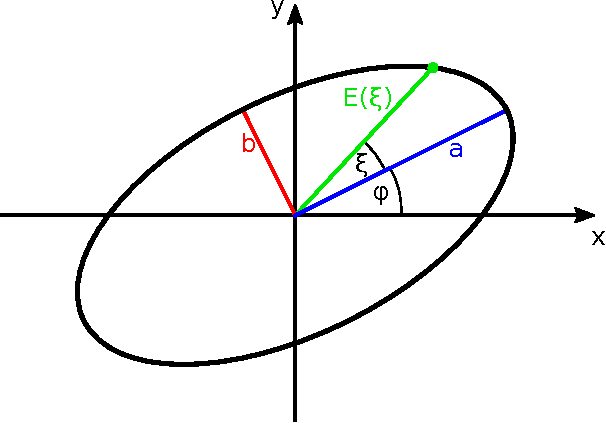
\includegraphics{img/ellipse_sketch.pdf}
 \caption{A general ellipse can be described by the lengths of its two half-axes~$a$ and~$b$
 and two angles, namely the rotation angle of the major half-axis~$\varphi$
 and the tangential origin~$\xi$.}
 \label{fig:ellipse_sketch}
\end{figure}
Alternatively, any ellipse can also be described by the lengths of its two half-axes~$a$ and~$b$
and two angles~$\varphi$ and~$\xi$ (see Fig.~\ref{fig:ellipse_sketch}).
It turns out that yet another parameterization
in terms of three Fourier coefficients~$\hat{c}$, $\hat{s}$ and~$\hat{r}$ plus one angle~$\Delta \theta$ is possible.
We focus only on the $m=1$-contribution for now:
\begin{align}
 x_1(\theta) =&\, \hat{c} \cos(\theta + \Delta \theta) + \hat{r} \sin(\theta + \Delta \theta) \label{eqn:ellipse_4_x} \\
 y_1(\theta) =&\, \hat{s} \sin(\theta + \Delta \theta) + \hat{r} \cos(\theta + \Delta \theta) \label{eqn:ellipse_4_y} \, .
\end{align}
The shape of the ellipse in realspace is completely determined by three parameters,
which in terms of Fig.~\ref{fig:ellipse_sketch} would be the set~$\{a, b, \varphi\}$.
The fourth parameter sets the origin for the tangential coordinate.
Varying it only shifts points back and forth along the circumference of the ellipse,
but does not change its general appearance.
It should be noted that the poloidal origin is the same for all contributions
to the Fourier representation of the surface.
Consequently, fixing the poloidal origin for any one of the various-$m$ contributions
implicitly defines the poloidal origin also for all other-$m$ contributions.
This is put to use when finding a spectrally-condensed Fourier representation
for a given surface geometry.
Here, the $m=1$ - contribution is reparameterized according to~\eqn{ellipse_4_x} and~\eqn{ellipse_4_y}
with the tangential offset~$\Delta \theta$ assumed to be zero,
which leads to an implicit determination of the tangential origin:
\begin{align}
 x_1(\theta) =&\, \hat{c} \cos(\theta) + \hat{r} \sin(\theta) \label{eqn:ellipse_3_x} \\
 y_1(\theta) =&\, \hat{s} \sin(\theta) + \hat{r} \cos(\theta) \label{eqn:ellipse_3_y} \, .
\end{align}

Summarizing, the set of Fourier coefficients to describe a given surface geometry
is reduced by one element by assuming~$\hat{x}_1^\mathrm{s} = \hat{y}_1^\mathrm{c}$
and by this constraint on the $m=1$ - contribution,
the location of the tangential origin is implictly defined.
All other-$m$ contributions retain their full set of four Fourier coefficients.

It might be useful for one or the other purpose to know the $\{\hat{c}, \hat{s}, \hat{r}, \Delta \theta \}$-representation
of an ellipse specified in terms of the regular four
Fourier coefficients~$\{\hat{x}_1^\mathrm{c}, \hat{x}_1^\mathrm{s}, \hat{y}_1^\mathrm{c}, \hat{y}_1^\mathrm{s}\}$.
This is done next.
We start by considering the representation of an ellipse by~\eqn{ellipse_4_x} and~\eqn{ellipse_4_y}:
\begin{align}
                ~&\, \begin{cases}
                       x_1(\theta) =&\, \hat{c} \cos(\theta + \Delta \theta) + \hat{r} \sin(\theta + \Delta \theta) \\
                       y_1(\theta) =&\, \hat{s} \sin(\theta + \Delta \theta) + \hat{r} \cos(\theta + \Delta \theta)
                     \end{cases} \nonumber \\
 \Leftrightarrow &\, \begin{cases}
                       x_1(\theta) =&\,   \hat{c} \left[ \cos(\theta) \cos(\Delta \theta) - \sin(\theta) \sin(\Delta \theta) \right]
                                        + \hat{r} \left[ \sin(\theta) \cos(\Delta \theta) + \cos(\theta) \sin(\Delta \theta) \right]  \\
                       y_1(\theta) =&\,   \hat{s} \left[ \sin(\theta) \cos(\Delta \theta) + \cos(\theta) \sin(\Delta \theta) \right]
                                        + \hat{r} \left[ \cos(\theta) \cos(\Delta \theta) - \sin(\theta) \sin(\Delta \theta) \right]
                     \end{cases} \nonumber \\
 \Leftrightarrow &\, \begin{cases}
                       x_1(\theta) =&\,   \cos(\theta) \left[             \hat{c} \cos(\Delta \theta) + \hat{r} \sin(\Delta \theta) \right]
                                        + \sin(\theta) \left[          -  \hat{c} \sin(\Delta \theta) + \hat{r} \cos(\Delta \theta) \right] \\
                       y_1(\theta) =&\,   \sin(\theta) \left[             \hat{s} \cos(\Delta \theta) - \hat{r} \sin(\Delta \theta) \right]
                                        + \cos(\theta) \left[ \phantom{-} \hat{s} \sin(\Delta \theta) + \hat{r} \cos(\Delta \theta) \right]
                     \end{cases}
\end{align}
Equating coefficients with~\eqn{x_m_contrib} and~\eqn{y_m_contrib}, we find:
\begin{align}
 \hat{x}_1^\mathrm{c} =&\, \phantom{-}~ \hat{c} \cos(\Delta \theta) + \hat{r} \sin(\Delta \theta) \\
 \hat{x}_1^\mathrm{s} =&\,          -   \hat{c} \sin(\Delta \theta) + \hat{r} \cos(\Delta \theta) \\
 \hat{y}_1^\mathrm{c} =&\, \phantom{-}~ \hat{r} \cos(\Delta \theta) + \hat{s} \sin(\Delta \theta) \\
 \hat{y}_1^\mathrm{s} =&\,          -   \hat{r} \sin(\Delta \theta) + \hat{s} \cos(\Delta \theta)
\end{align}
or equally in matrix form:
\begin{align}
 \begin{pmatrix}
  \hat{x}_1^\mathrm{c} \\
  \hat{x}_1^\mathrm{s}
 \end{pmatrix}
 =&\,
 \mathbf{R}(\Delta \theta)
 \begin{pmatrix}
  \hat{c} \\
  \hat{r}
 \end{pmatrix} \\
 \begin{pmatrix}
  \hat{y}_1^\mathrm{c} \\
  \hat{y}_1^\mathrm{s}
 \end{pmatrix}
 =&\,
 \mathbf{R}(\Delta \theta)
 \begin{pmatrix}
  \hat{r} \\
  \hat{s}
 \end{pmatrix}
\end{align}
with the rotation matrix~$\mathbf{R}(\Delta \theta)$:
\begin{equation}
 \mathbf{R}(\Delta \theta)
 = \begin{pmatrix}
    \phantom{-}\, \cos(\Delta \theta) & \sin(\Delta \theta) \\
             -    \sin(\Delta \theta) & \cos(\Delta \theta)
   \end{pmatrix} \, .
\end{equation}
The rotation matrix is readily inverted by observing:
\begin{equation}
 \mathbf{R}^{-1}(\Delta \theta) = \mathbf{R}(-\Delta \theta) \, ,
\end{equation}
leading to:
\begin{equation}
 \mathbf{R}^{-1}(\Delta \theta)
 = \begin{pmatrix}
    \cos(\Delta \theta) &          -    \sin(\Delta \theta) \\
    \sin(\Delta \theta) & \phantom{-}\, \cos(\Delta \theta)
   \end{pmatrix} \, .
\end{equation}
This allows us to obtain the three-parameter representation for the ellipse
given the standard four Fourier coefficients and assuming $\Delta \theta$ is known already:
\begin{align}
 \begin{pmatrix}
  \hat{c} \\
  \hat{r}
 \end{pmatrix}
 =&\,
 \mathbf{R}^{-1}(\Delta \theta)
 \begin{pmatrix}
  \hat{x}_1^\mathrm{c} \\
  \hat{x}_1^\mathrm{s}
 \end{pmatrix} \label{eqn:cr_from_x1cs} \\
 \begin{pmatrix}
  \hat{r} \\
  \hat{s}
 \end{pmatrix}
 =&\,
 \mathbf{R}^{-1}(\Delta \theta)
 \begin{pmatrix}
  \hat{y}_1^\mathrm{c} \\
  \hat{y}_1^\mathrm{s}
 \end{pmatrix} \label{eqn:rs_from_y1cs} \, .
\end{align}
We note that this way we have two expressions for the shared Fourier coefficient~$\hat{r}$:
\begin{align}
 \hat{r} =&\, \hat{x}_1^\mathrm{c} \sin(\Delta \theta) + \hat{x}_1^\mathrm{s} \cos(\Delta \theta) \\
 \hat{r} =&\, \hat{y}_1^\mathrm{c} \cos(\Delta \theta) - \hat{y}_1^\mathrm{s} \sin(\Delta \theta) \, .
\end{align}
These two expressions can be equated and solved for the so-far unknown $\Delta \theta$:
\begin{align}
                 \hat{x}_1^\mathrm{c} \sin(\Delta \theta) + \hat{x}_1^\mathrm{s} \cos(\Delta \theta)
            =&\, \hat{y}_1^\mathrm{c} \cos(\Delta \theta) - \hat{y}_1^\mathrm{s} \sin(\Delta \theta) \nonumber \\
 \Leftrightarrow \sin(\Delta \theta) \left[ \hat{x}_1^\mathrm{c} + \hat{y}_1^\mathrm{s} \right]
            +&\, \cos(\Delta \theta) \left[ \hat{x}_1^\mathrm{s} - \hat{y}_1^\mathrm{c} \right] = 0 \nonumber \\
 \Leftrightarrow \frac{\sin(\Delta \theta)}{\cos(\Delta \theta)}
            =&\, \frac{\hat{y}_1^\mathrm{c} - \hat{x}_1^\mathrm{s}}{\hat{x}_1^\mathrm{c} + \hat{y}_1^\mathrm{s}} \nonumber \\
 \Leftrightarrow \Delta \theta
            =&\, \arctan\left( \frac{\hat{y}_1^\mathrm{c} - \hat{x}_1^\mathrm{s}}{\hat{x}_1^\mathrm{c} + \hat{y}_1^\mathrm{s}} \right) \label{eqn:delta_theta_ellipse_3} \, .
\end{align}
A possible division by zero can be circumvented by evaluating \eqn{delta_theta_ellipse_3} using the \texttt{arctan2} function:
\begin{equation}
 \boxed{\Delta \theta = \texttt{arctan2}\left(\hat{y}_1^\mathrm{c} - \hat{x}_1^\mathrm{s}, \hat{x}_1^\mathrm{c} + \hat{y}_1^\mathrm{s}\right)} \, .
\end{equation}
The other coefficients~$\hat{c}$, $\hat{s}$ and~$\hat{r}$ can then be obtained
from the original four Fourier coefficients
using \eqn{cr_from_x1cs} and \eqn{rs_from_y1cs}.
There is one last ambiguity.
The tangential origin displacement~$\Delta \theta$ is only unique up to a shift by $\pi$.
Thus, the following two representations yield geometrically equivalent ellipses:
\begin{equation}
 \{ \hat{c}, \hat{s}, \hat{r}, \Delta \theta \} \textrm{ and } \{ -\hat{c}, -\hat{s}, -\hat{r}, \Delta \theta + \pi \} \, .
\end{equation}
They differ by the poloidal origin being displaced to the opposite side of the ellipse,
similar to the illustration in Fig.~8c in Ref.~\cite{kuhl_giardina_1982}.
